\documentclass{beamer}

\RequirePackage{xparse}

%% https://www.quora.com/Presentations-What-are-the-best-beamer-themes
\setbeamertemplate{frametitle}
  {\begin{centering}\smallskip
   \insertframetitle\par
   \smallskip\end{centering}}
\setbeamertemplate{itemize item}{\(\bullet\)}
\setbeamertemplate{navigation symbols}{}
\setbeamertemplate{footline}[text line]{%
    \hfill\strut{%
        \scriptsize\sf\color{black!60}%
        \quad\insertframenumber
    }%
    \hfill
}

\definecolor{NoteBrown}{RGB}{152,101,47}
\definecolor{NoteBlue}{RGB}{31,91,255}
\definecolor{NoteGreen}{RGB}{62,195,74}
\definecolor{NoteRed}{RGB}{191,0,0}
\definecolor{NotePurple}{RGB}{151,54,208}
\definecolor{NoteDarkGreen}{RGB}{0,121,62}
\definecolor{NoteGrey}{RGB}{150,150,150}
\definecolor{NoteOrange}{RGB}{255,155,0}

% Define some colors:
\definecolor{PittBlue}{RGB}{0,43,94}
\definecolor{PittGold}{RGB}{197,168,118}
\definecolor{DarkFern}{HTML}{407428}
\definecolor{DarkCharcoal}{HTML}{4D4944}
\colorlet{Fern}{DarkFern!85!white}
\colorlet{Charcoal}{DarkCharcoal!85!white}
\colorlet{LightCharcoal}{Charcoal!50!white}
\colorlet{AlertColor}{orange!80!black}
\colorlet{DarkRed}{red!70!black}
\colorlet{DarkBlue}{blue!70!black}
\colorlet{DarkGreen}{green!70!black}
% Use the colors:
\setbeamercolor{title}{fg=PittBlue}
\setbeamercolor{frametitle}{fg=PittBlue}
\setbeamercolor{normal text}{fg=DarkCharcoal}
\setbeamercolor{block title}{fg=black,bg=Fern!25!white}
\setbeamercolor{block body}{fg=black,bg=Fern!25!white}
\setbeamercolor{alerted text}{fg=AlertColor}
\setbeamercolor{itemize item}{fg=Charcoal}

\usepackage[%
    backend    = biber,%
    style      = chem-acs,%
    autocite   = superscript,%
    backref    = true,%
    biblabel   = brackets,%
    doi        = true,%
    minnames   = 1,%
    maxnames   = 10,%
]{biblatex}
\addbibresource{../library.bib}
\addbibresource{../library2.bib}
\addbibresource{../paper_04/paper.bib}
\addbibresource{../paper_05/psi4numpy.bib}
\addbibresource{../paper_05/tutorial.bib}
\addbibresource{../5746059.bib}
\addbibresource{../5773968.bib}
\addbibresource{../in_preparation.bib}

\AtEveryCitekey{\iffootnote{\color{PittBlue}\tiny}{}}
\NewDocumentCommand{\nmfootfullcite}{m}{%
    \AtNextCite{%
        \let\thefootnote\relax
        \let\mkbibfootnote\mkbibfootnotetext
    }{%
        \footfullcite{#1}
    }
}

\RequirePackage{booktabs}
\RequirePackage{braket}
\RequirePackage{graphicx}
\RequirePackage{microtype}
\RequirePackage{minted}
\RequirePackage[version=4]{mhchem}
\RequirePackage{tabulary}

\NewDocumentCommand{\vect}{m}{%
        \ensuremath{\boldsymbol{\mathbf{#1}}}%
}%


\title{My Dissertation}
\author{Eric Berquist}
% \institute[Pitt]{Lambrecht Research Group \\ Dissertation Defense \\ \vspace{6pt} 
\includegraphics[width=1in]{./figures/pitt_logo.pdf}}
\institute{
\includegraphics[width=1in]{./figures/pitt_logo.pdf}}
\date{March 13th, 2018}

\begin{document}

\frame{
  \titlepage
}

\title{Decomposition of Intermolecular Interactions in \textit{Ab Initio} Spectroscopy}

\frame{
  \titlepage
}

\begin{frame}
  \frametitle{Goal of this work}
  It is possible to identify the contribution of specific molecular interaction to spectroscopic response
\end{frame}

\begin{frame}
  \frametitle{What is molecular response?}
  \begin{itemize}
  \item The experimentalist works at the \textcolor{green}{macroscopic level} and typically records the \textcolor{blue}{response of the electromagnetic field}.
  \item The theoretician works at the \textcolor{green}{microscopic level} and typically calculates the \textcolor{blue}{molecular response}.
  \item In order to connect experiment and theory we must reconcile these two different approaches.
  \end{itemize}
\end{frame}

% 0.35 for two side by side
\begin{frame}
  % \frametitle{\ce{CO2} asymmetric stretch lies in an isolated spectral window}
  \centering
  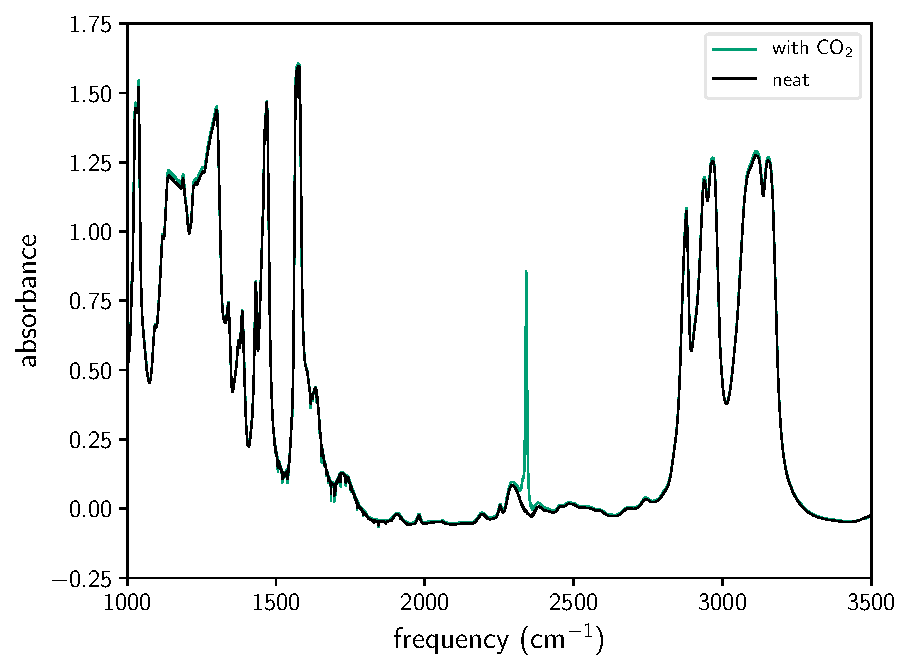
\includegraphics[scale=0.70]{./figures/experimental_spectra_TfO.pdf}
\end{frame}

\begin{frame}
  \centering
  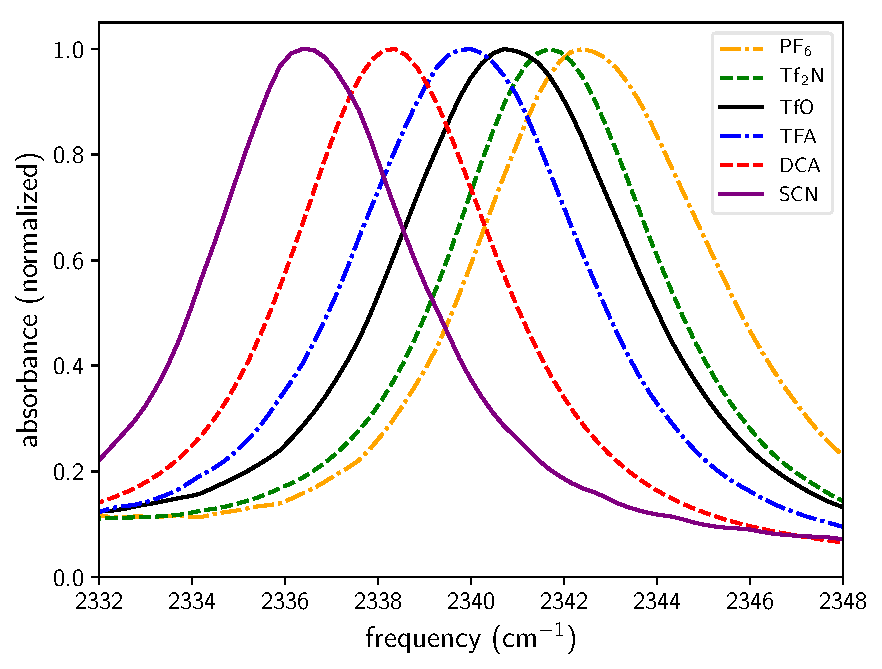
\includegraphics[scale=0.70]{./figures/experimental_spectra_shifting.pdf}
\end{frame}

\begin{frame}
  \centering
  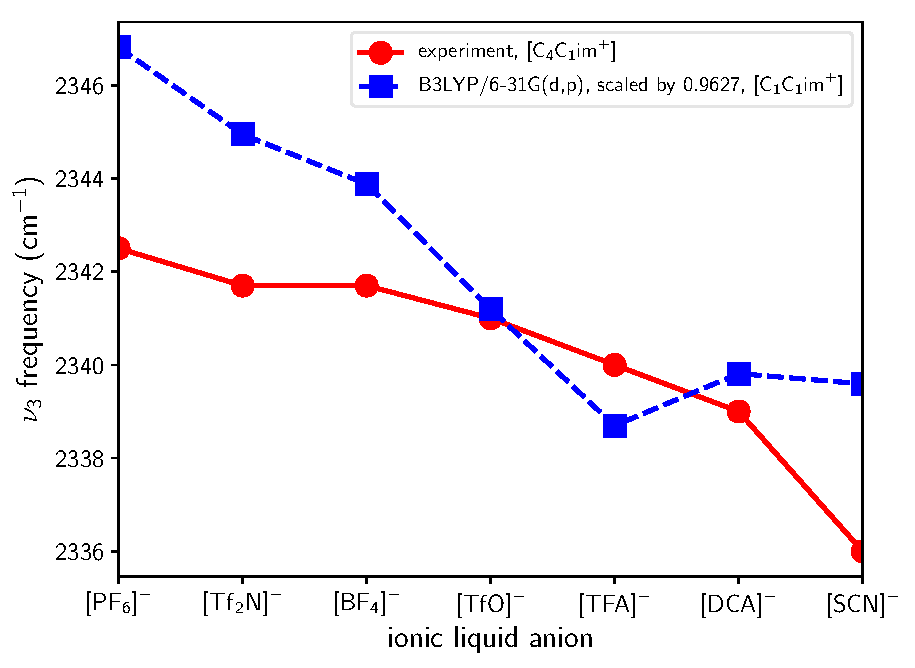
\includegraphics[scale=0.70]{./figures/frequencies_calc_vs_expt1.pdf}
  % \nmfootfullcite{Brinzer2015}
\end{frame}

% https://tex.stackexchange.com/q/157222/94717
\begin{frame}
  \begin{columns}
    \column{0.25\textwidth}
    \uncover<+->{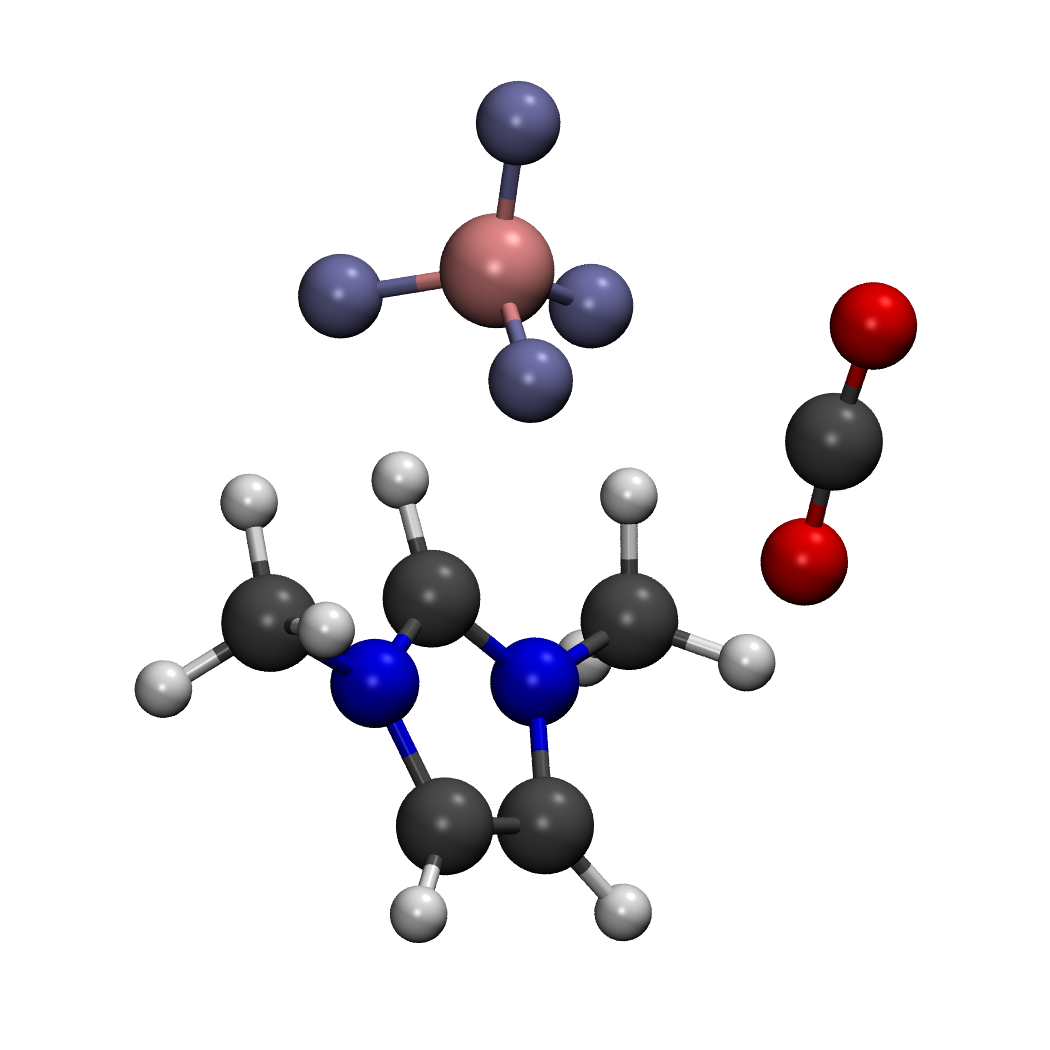
\includegraphics[scale=0.08]{./figures/cluster_BF4.png}}
    \uncover<.->{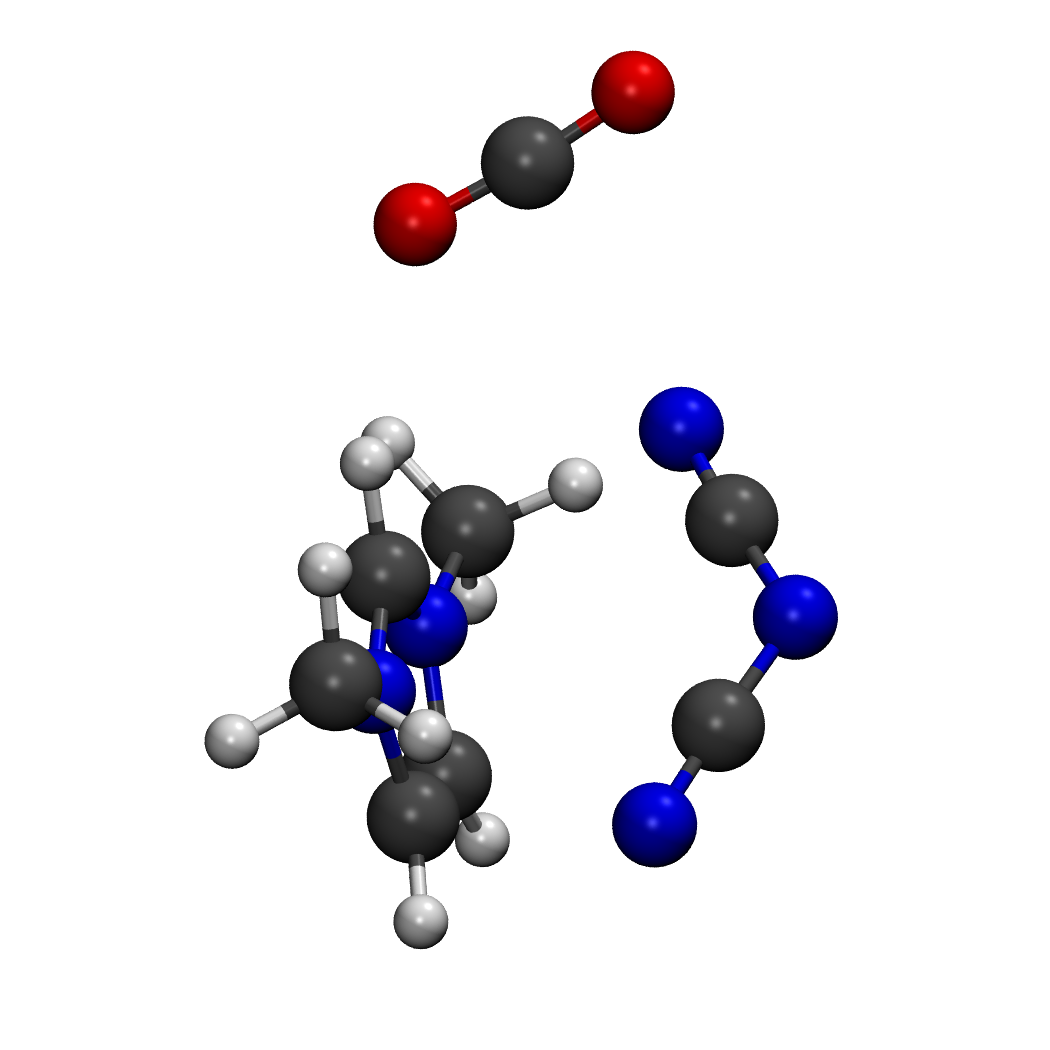
\includegraphics[scale=0.08]{./figures/cluster_DCA.png}}
    \column{0.25\textwidth}
    \uncover<.->{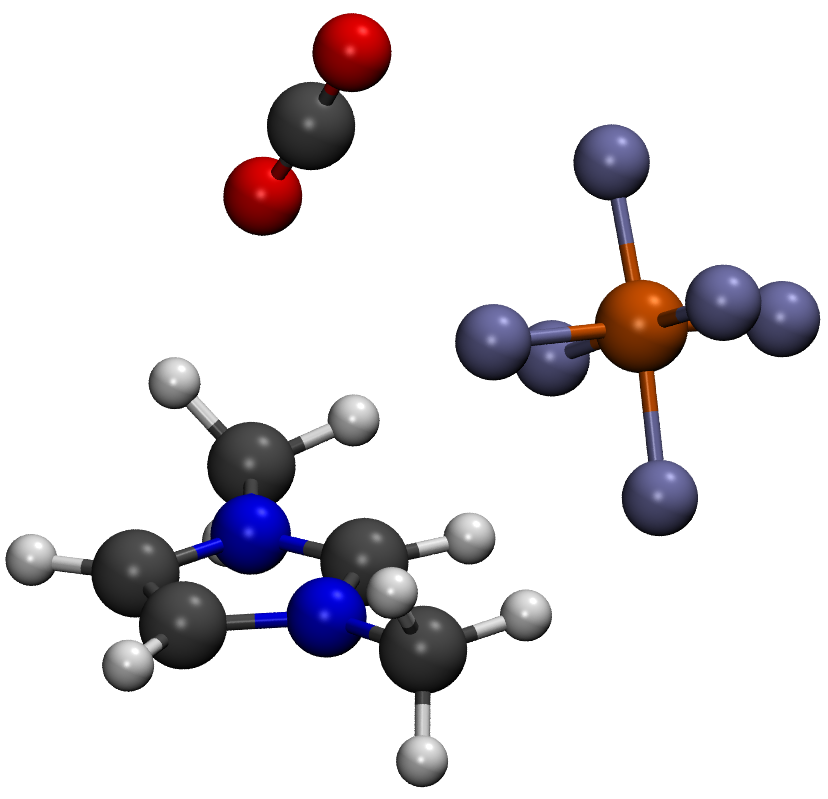
\includegraphics[scale=0.08]{./figures/cluster_PF6.png}}
    \uncover<.->{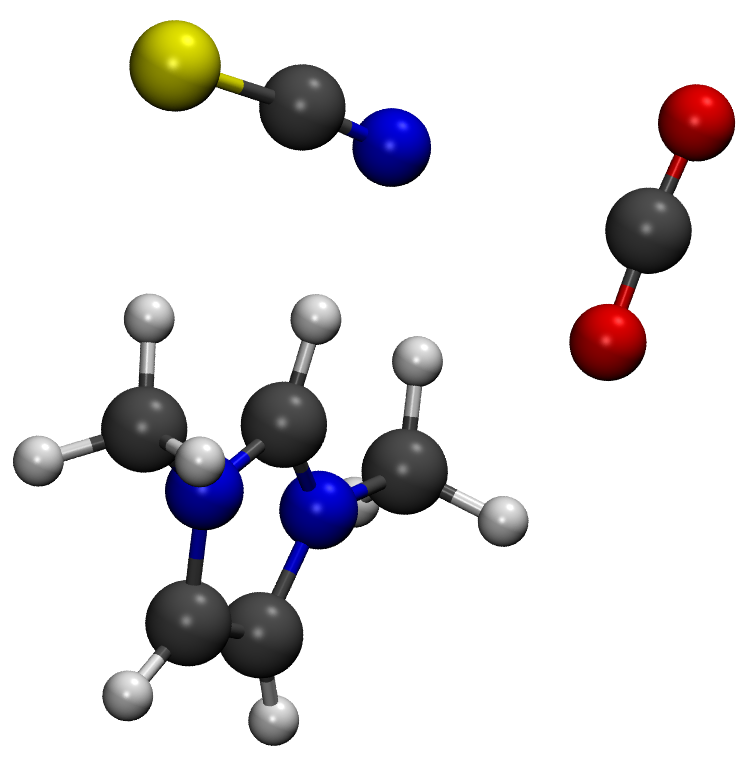
\includegraphics[scale=0.08]{./figures/cluster_SCN.png}}
    \column{0.25\textwidth}
    \uncover<.->{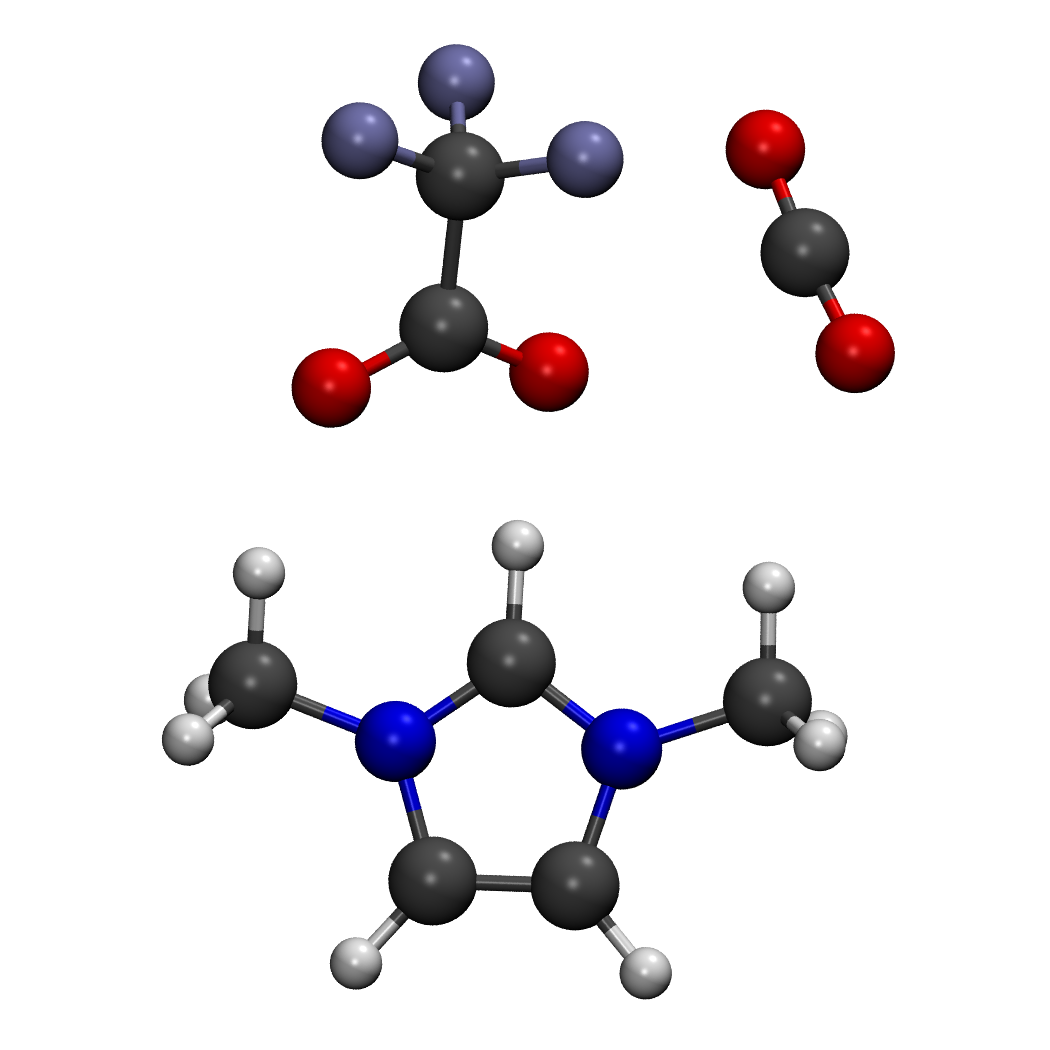
\includegraphics[scale=0.07]{./figures/cluster_TFA.png}}
    \uncover<.->{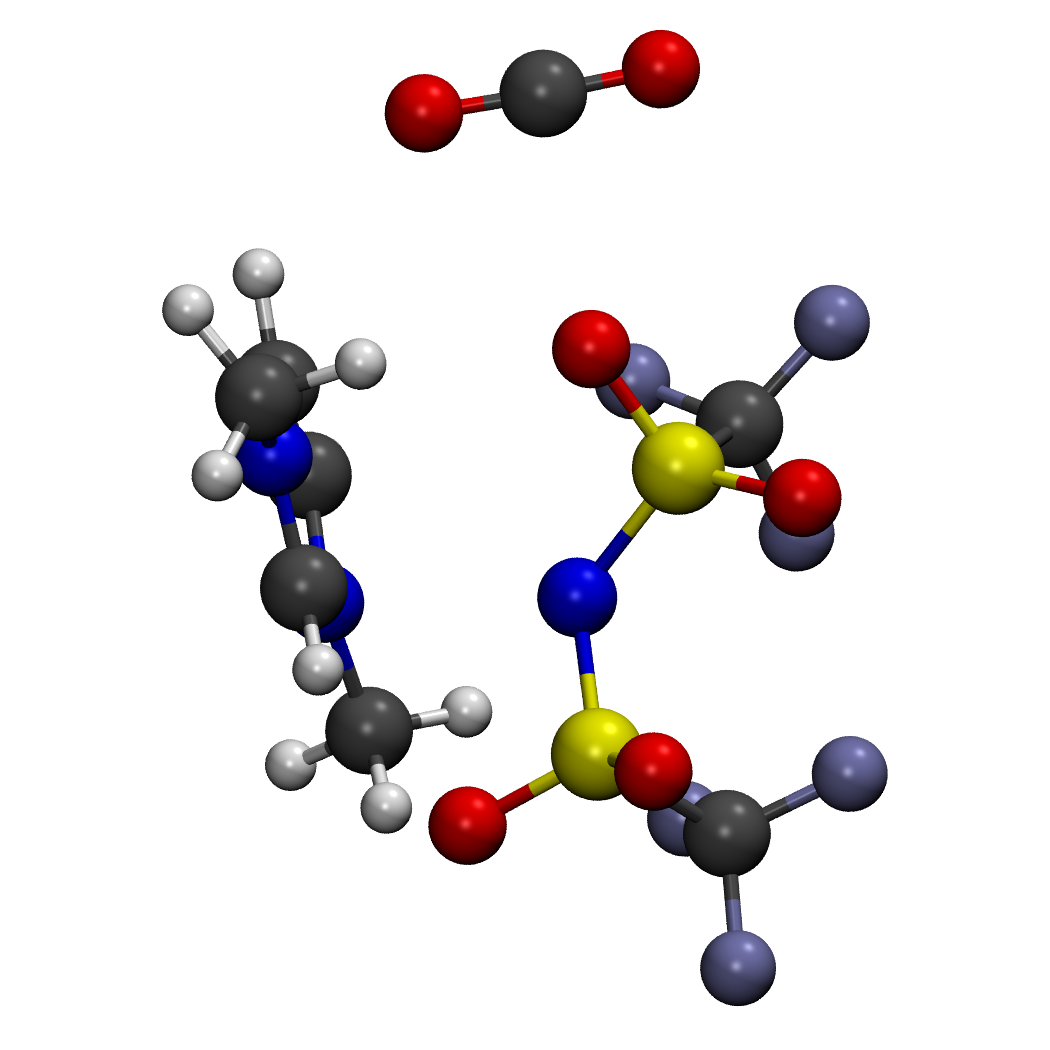
\includegraphics[scale=0.08]{./figures/cluster_Tf2N.png}}
    \column{0.25\textwidth}
    \uncover<.->{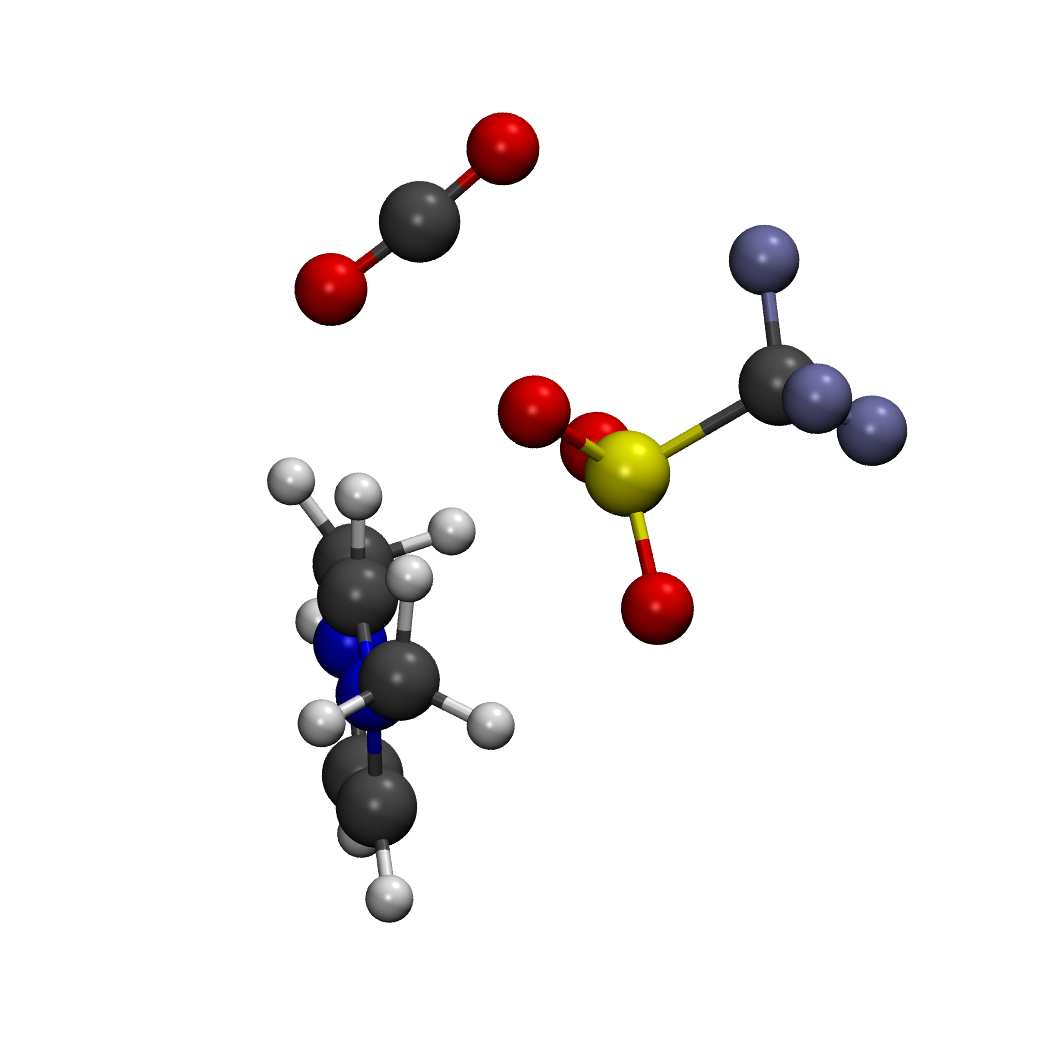
\includegraphics[scale=0.09]{./figures/cluster_TfO.png}}
  \end{columns}
  % \uncover<+->{}
\end{frame}

\begin{frame}
  \frametitle{ALMO-EDA}
  \centering
  \begin{equation*}
    \begin{aligned}
      E_{\text{tot}} &= E_{\text{free}} + \Delta E_{\text{int}} \\
      \Delta E_{\text{int}} &= \Delta E_{\text{gd}} + \Delta E_{\text{frz}} + \Delta E_{\text{pol}} + \Delta E_{\text{CT}}
    \end{aligned}
  \end{equation*}
  \uncover<1->{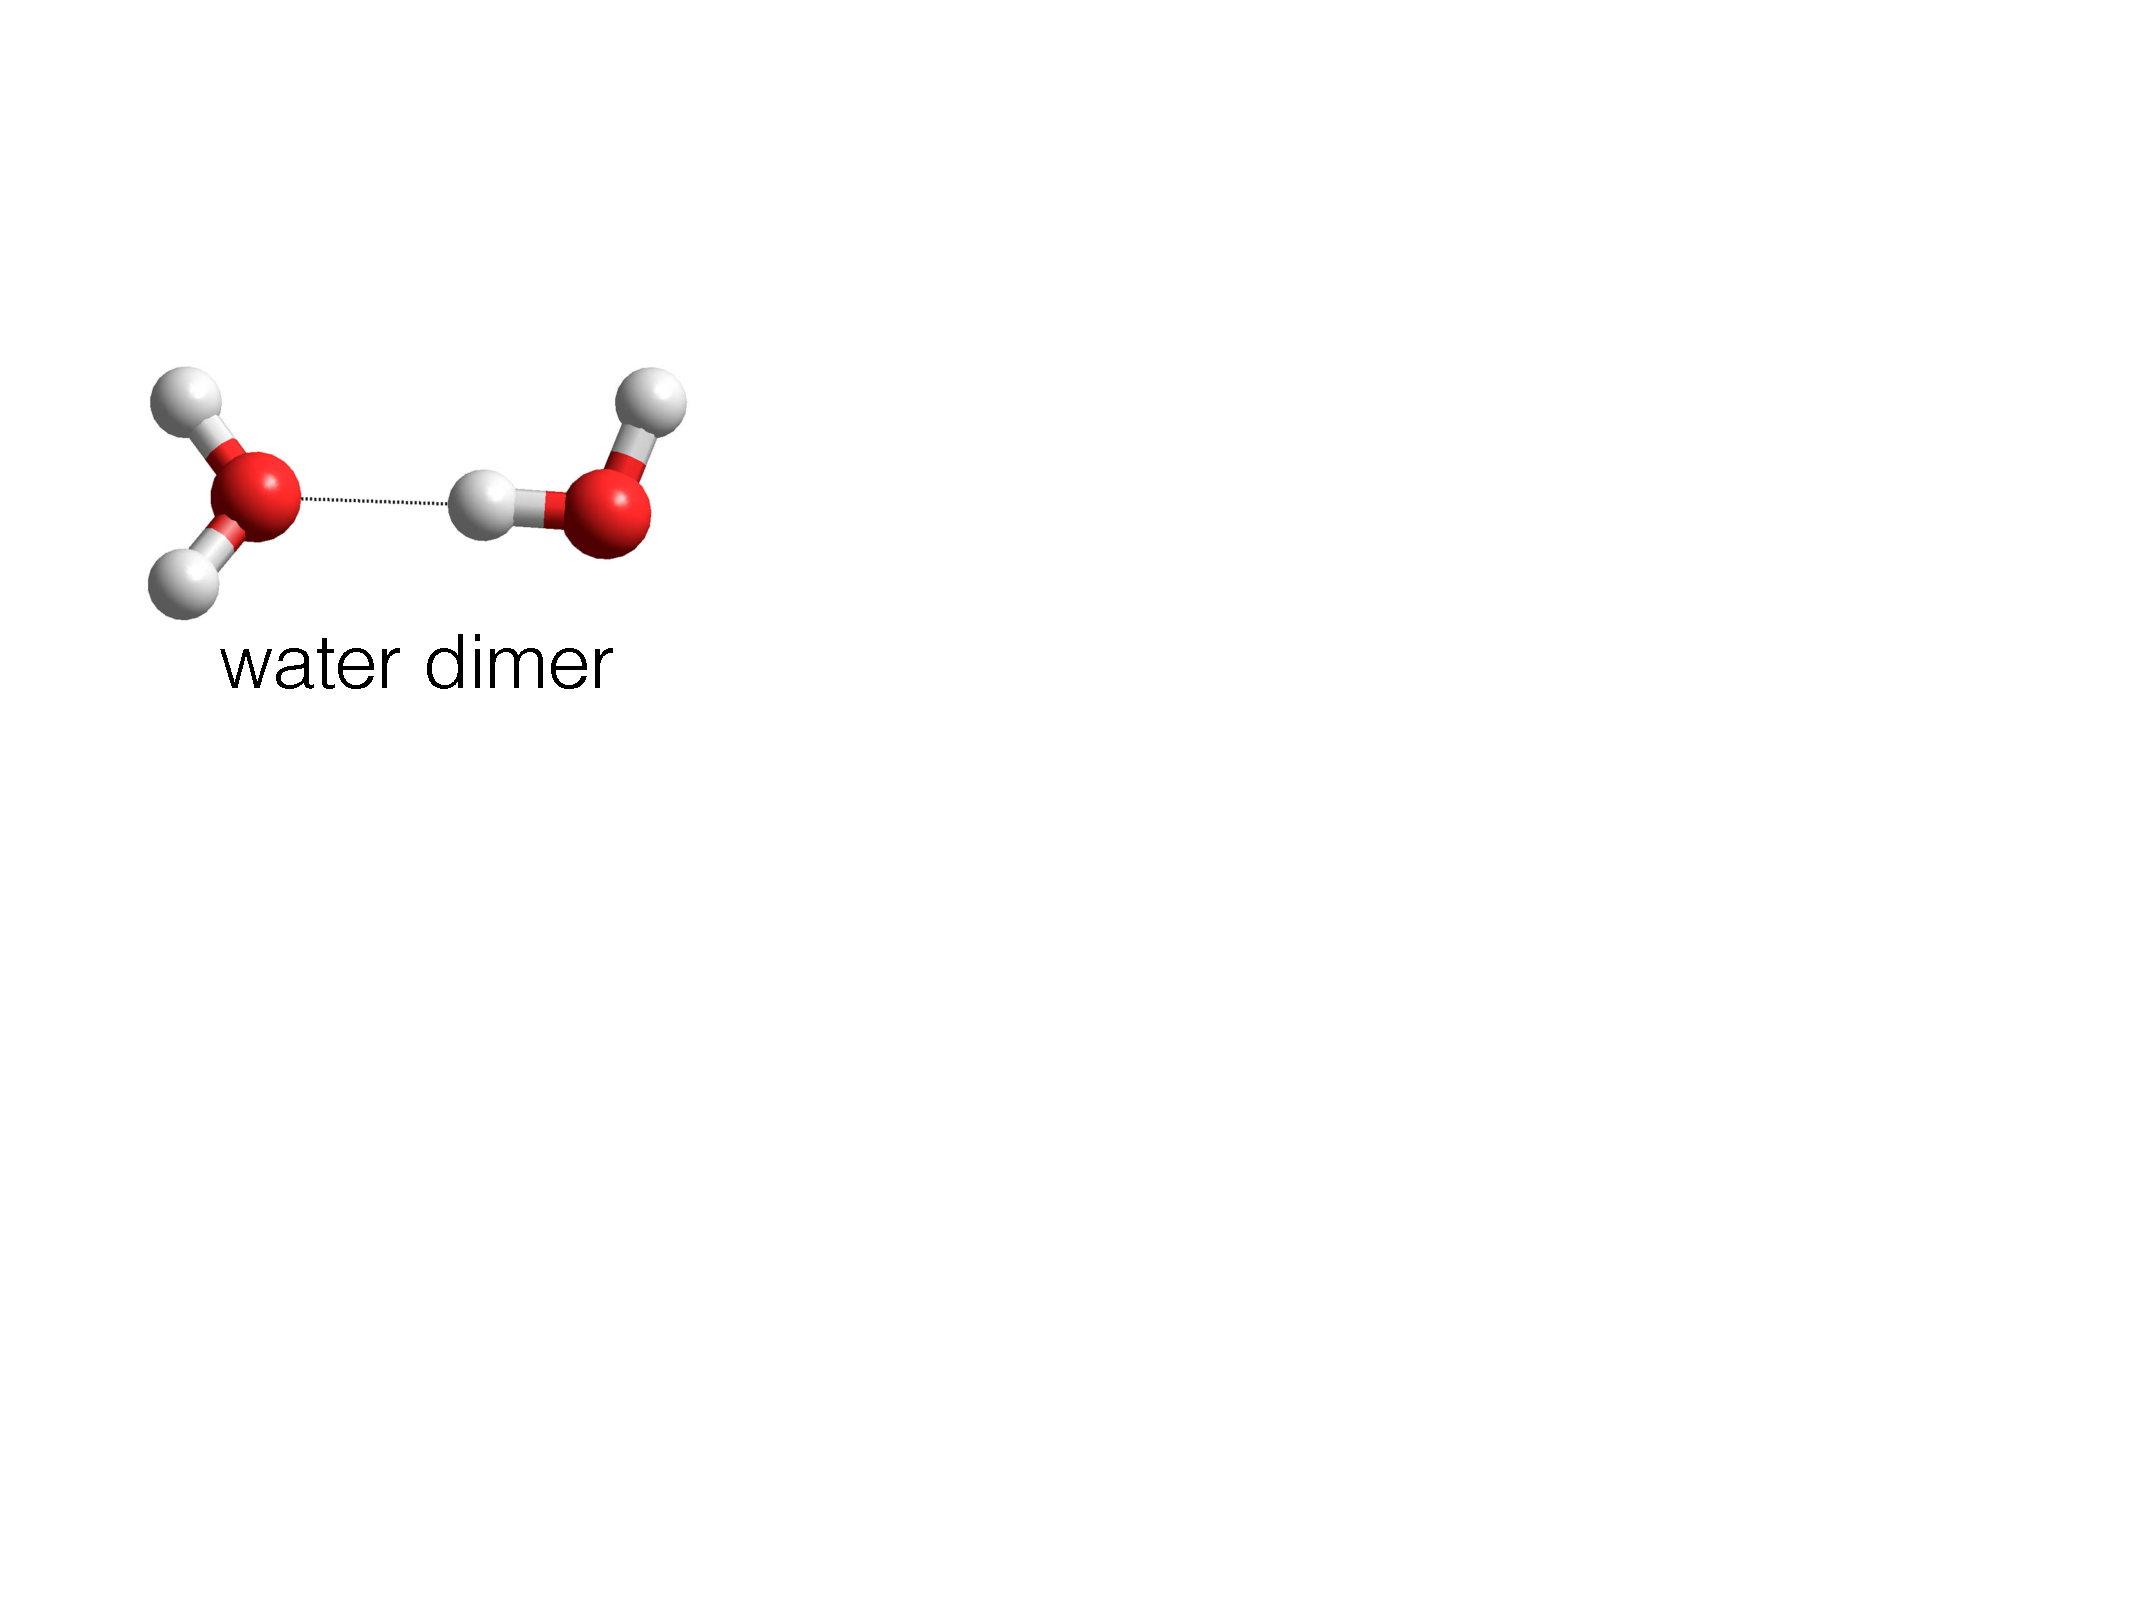
\includegraphics[scale=0.25]{./figures/almo_eda_00.pdf}}
  \uncover<2->{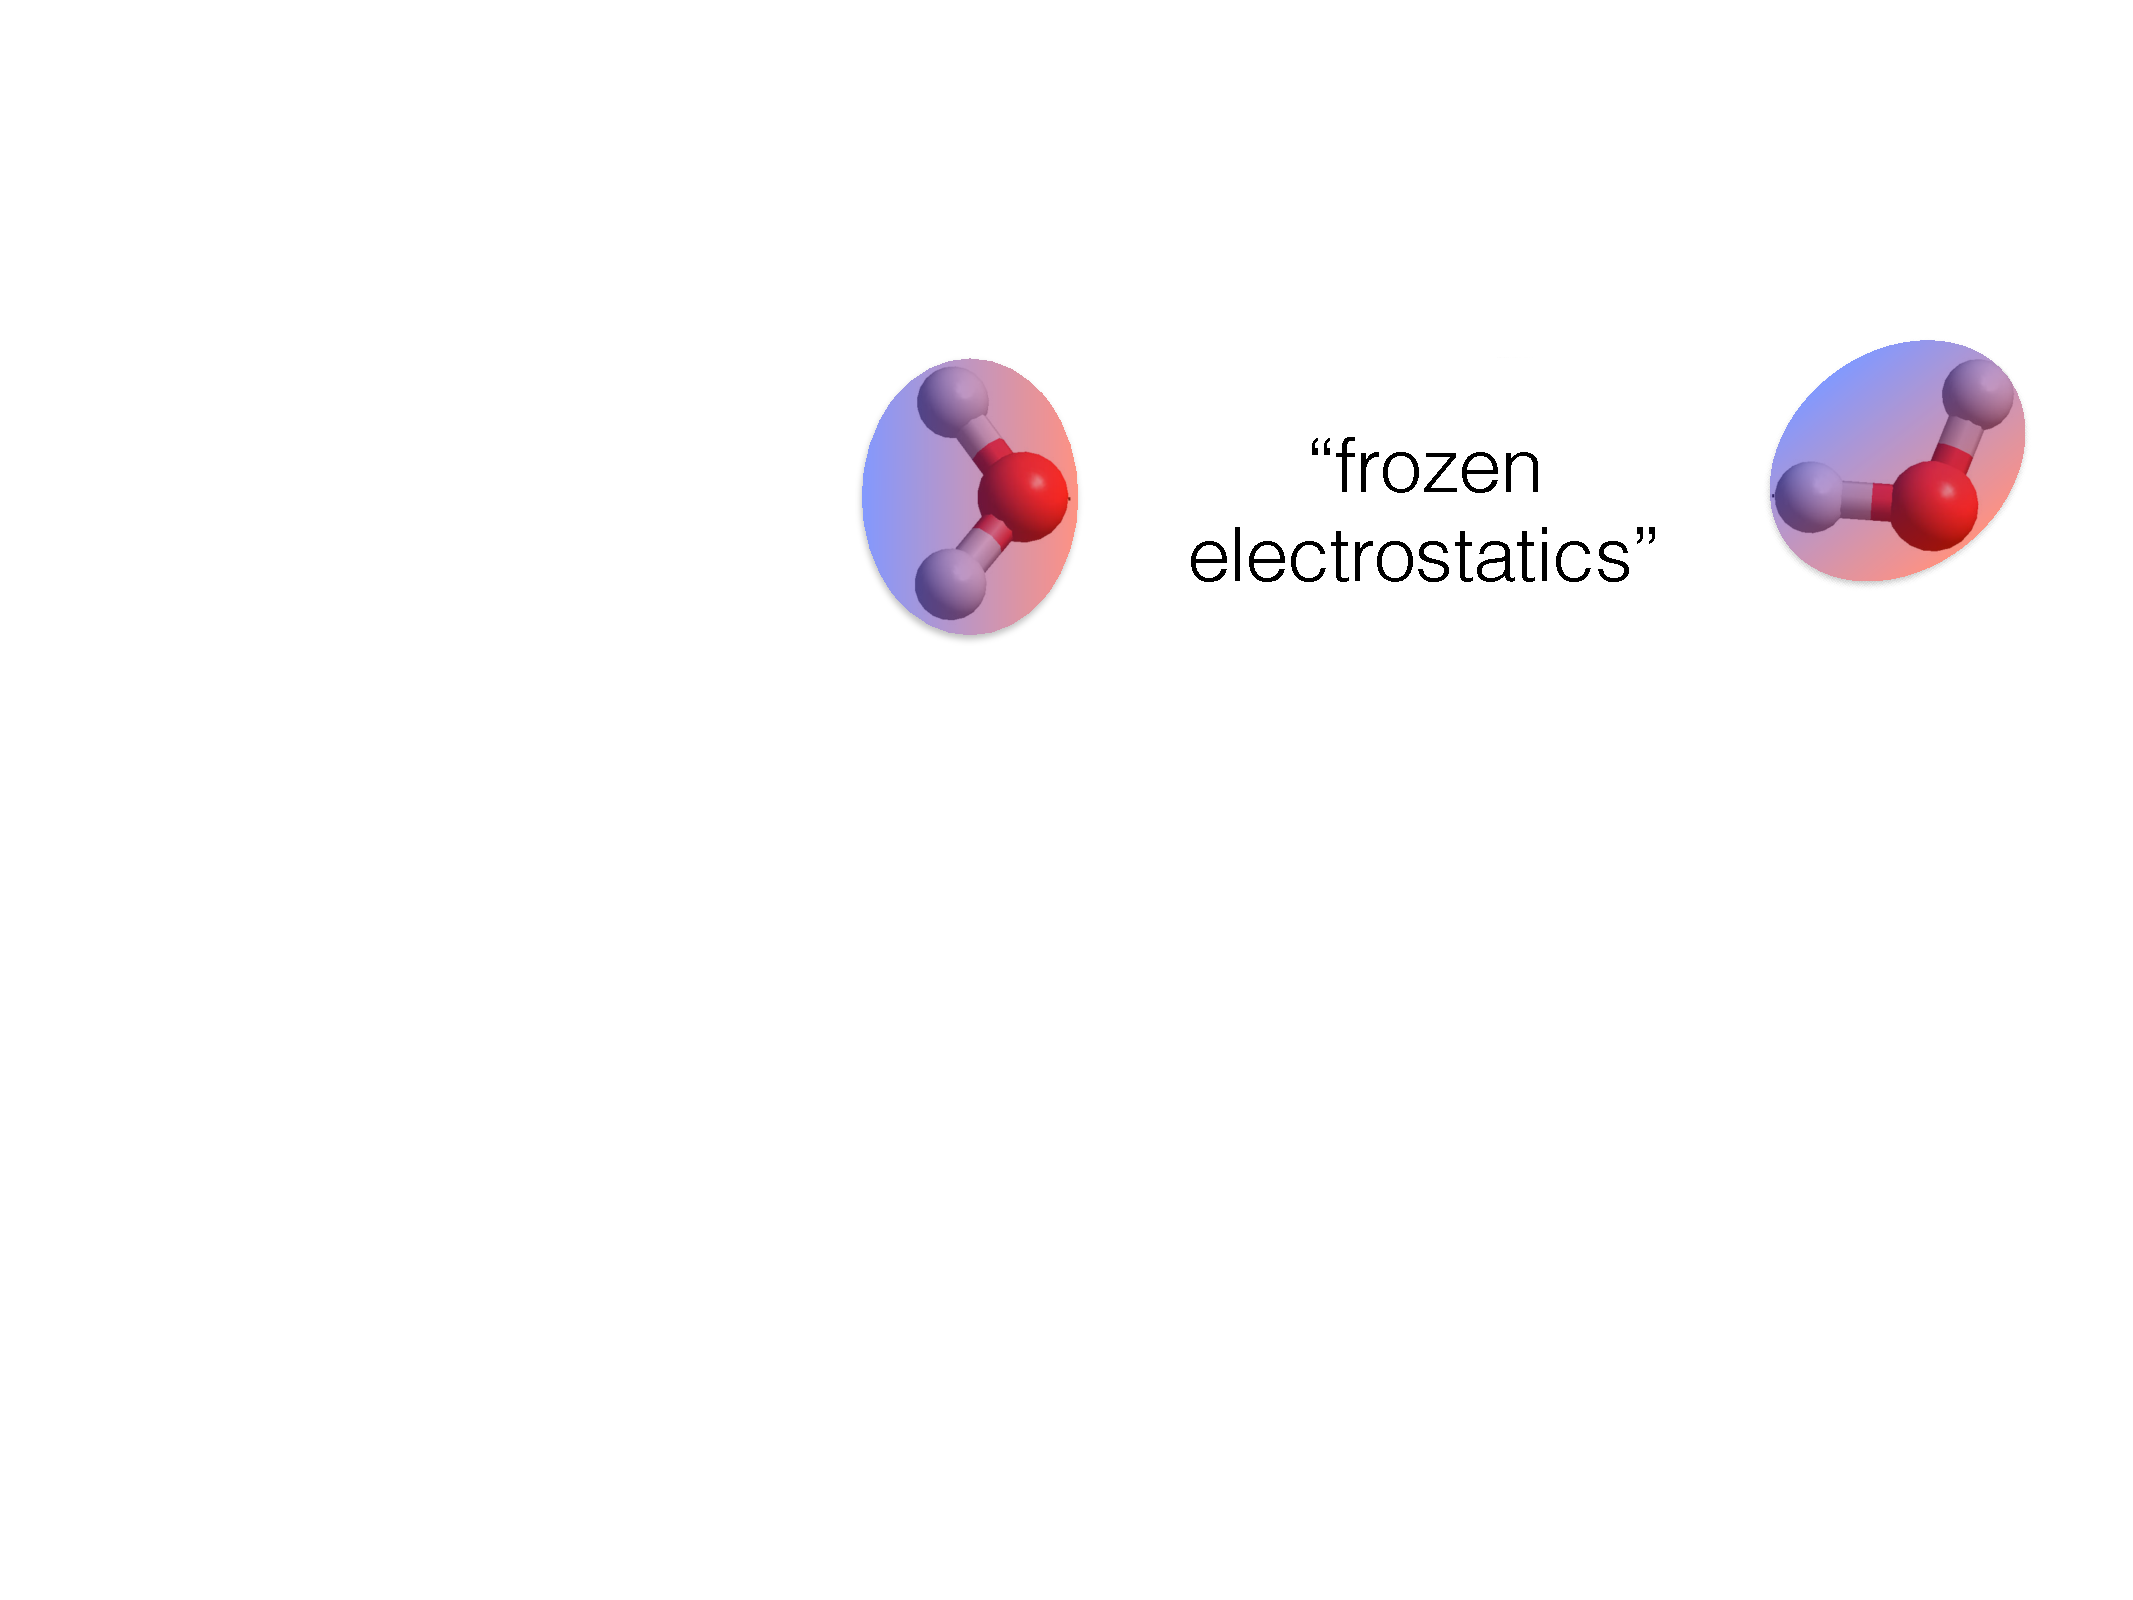
\includegraphics[scale=0.25]{./figures/almo_eda_02_frz.pdf}}
  \uncover<3->{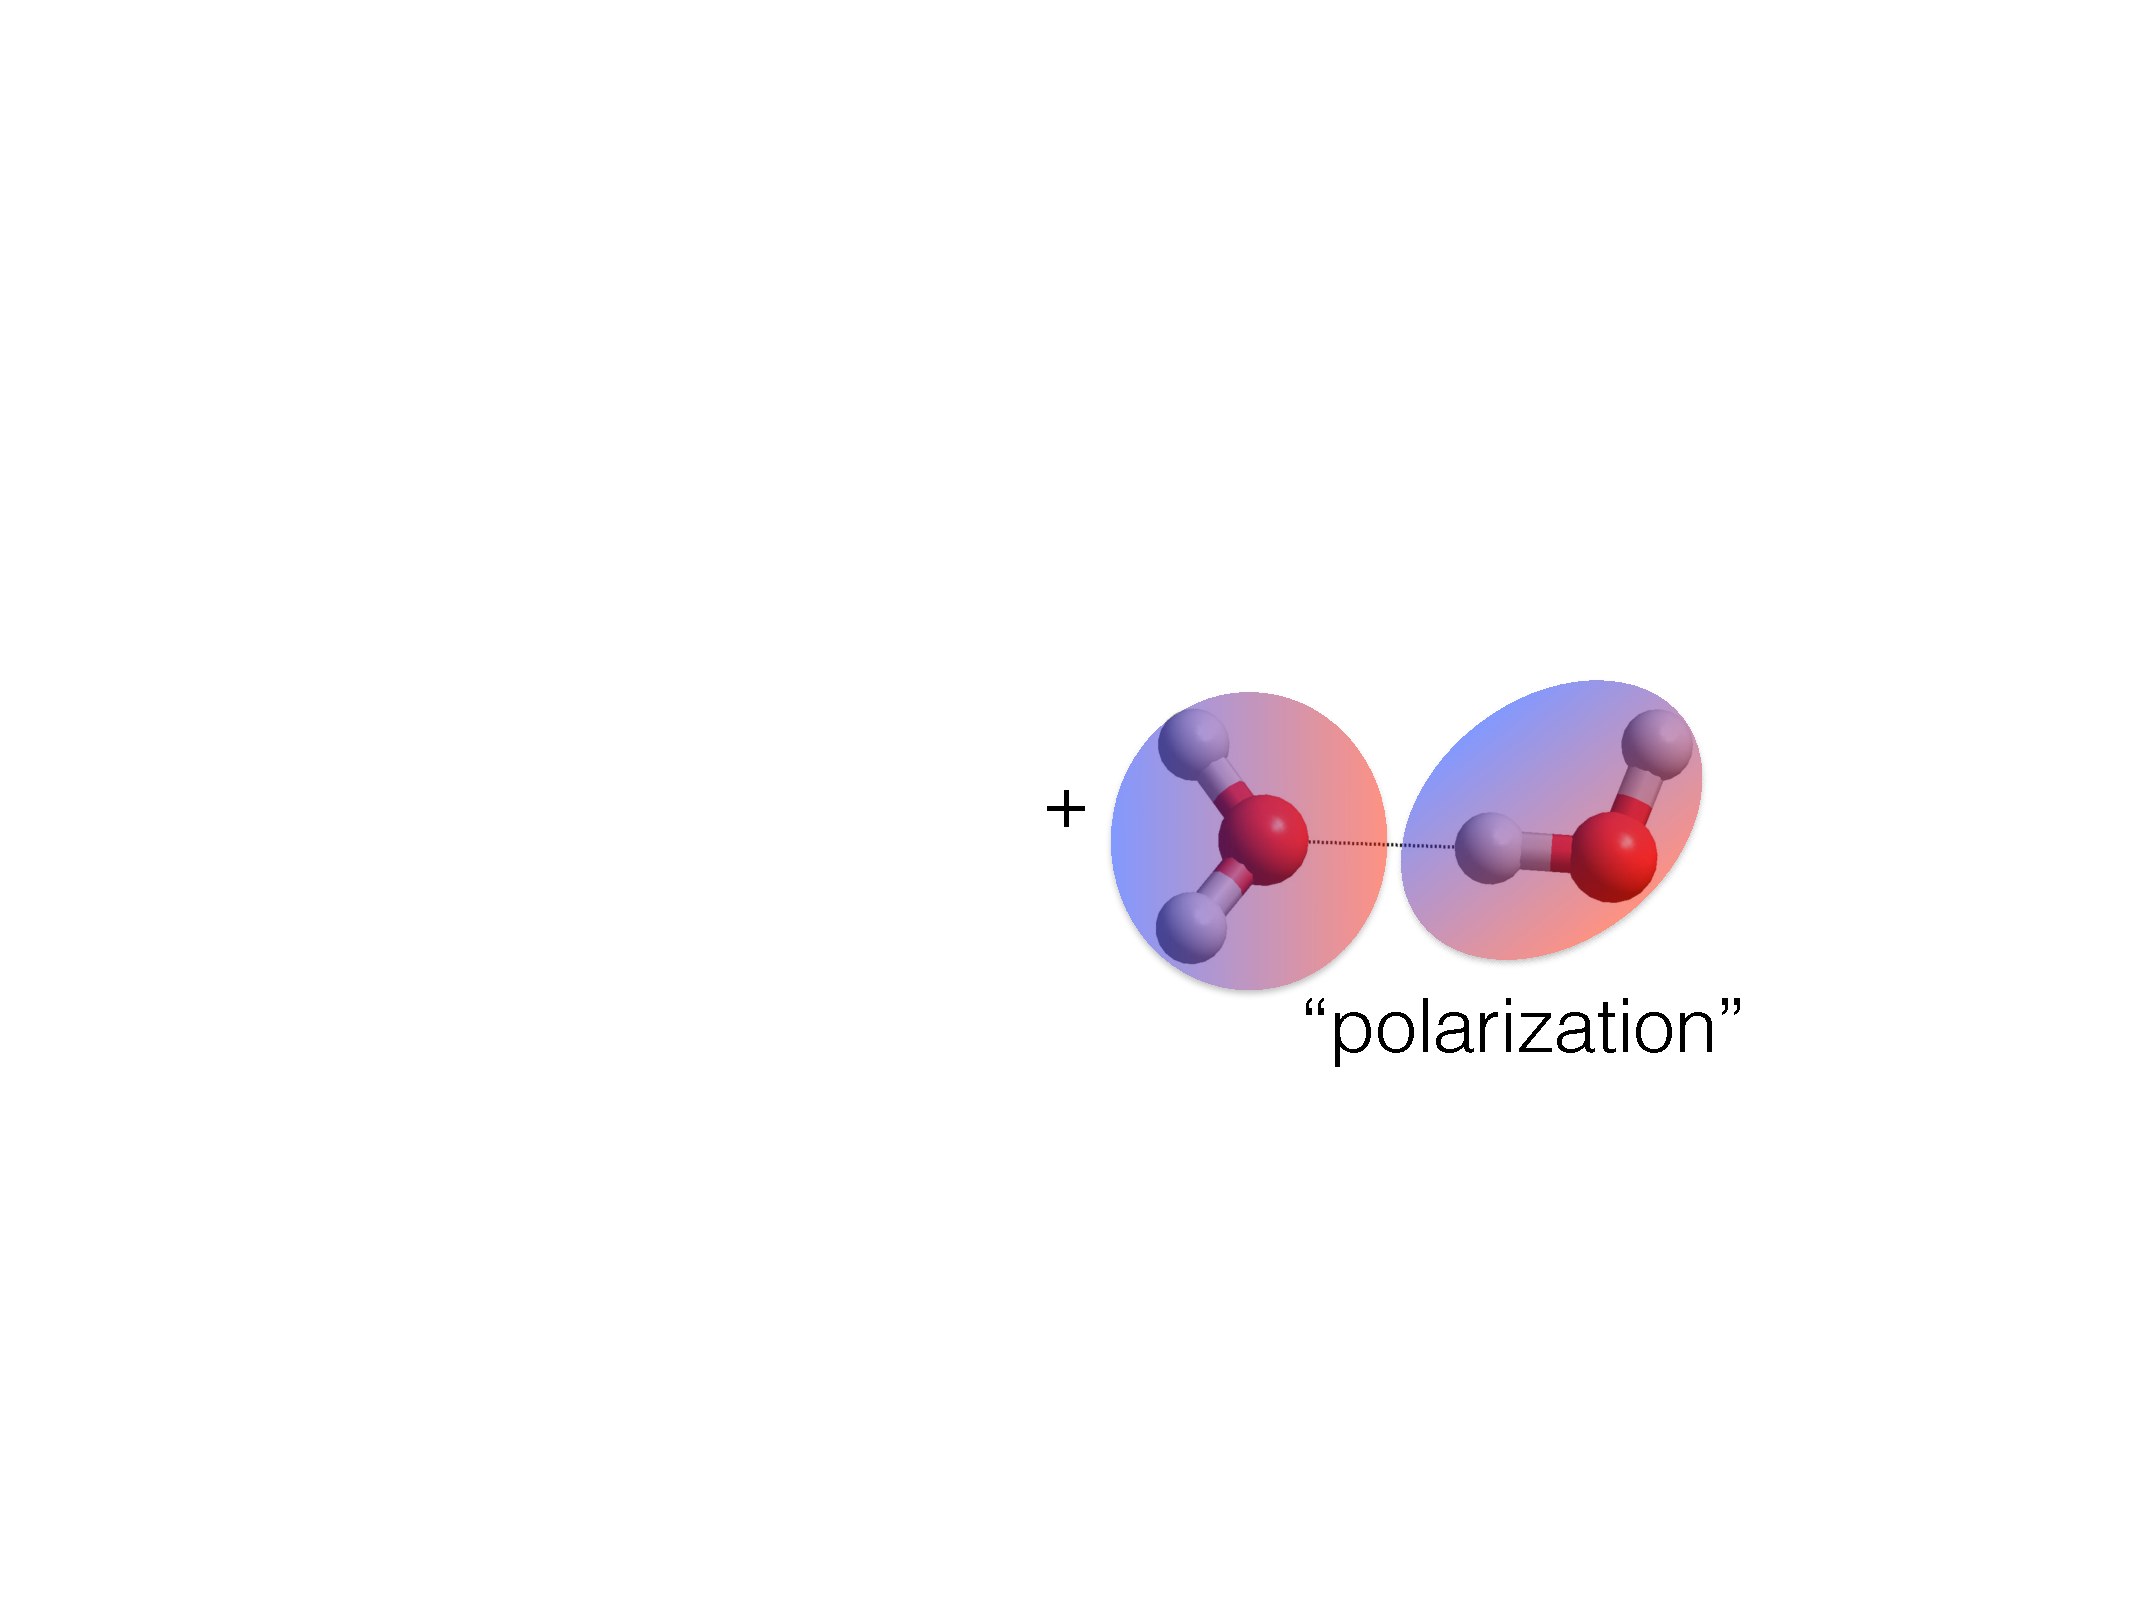
\includegraphics[scale=0.25]{./figures/almo_eda_03_pol.pdf}}
  \uncover<4->{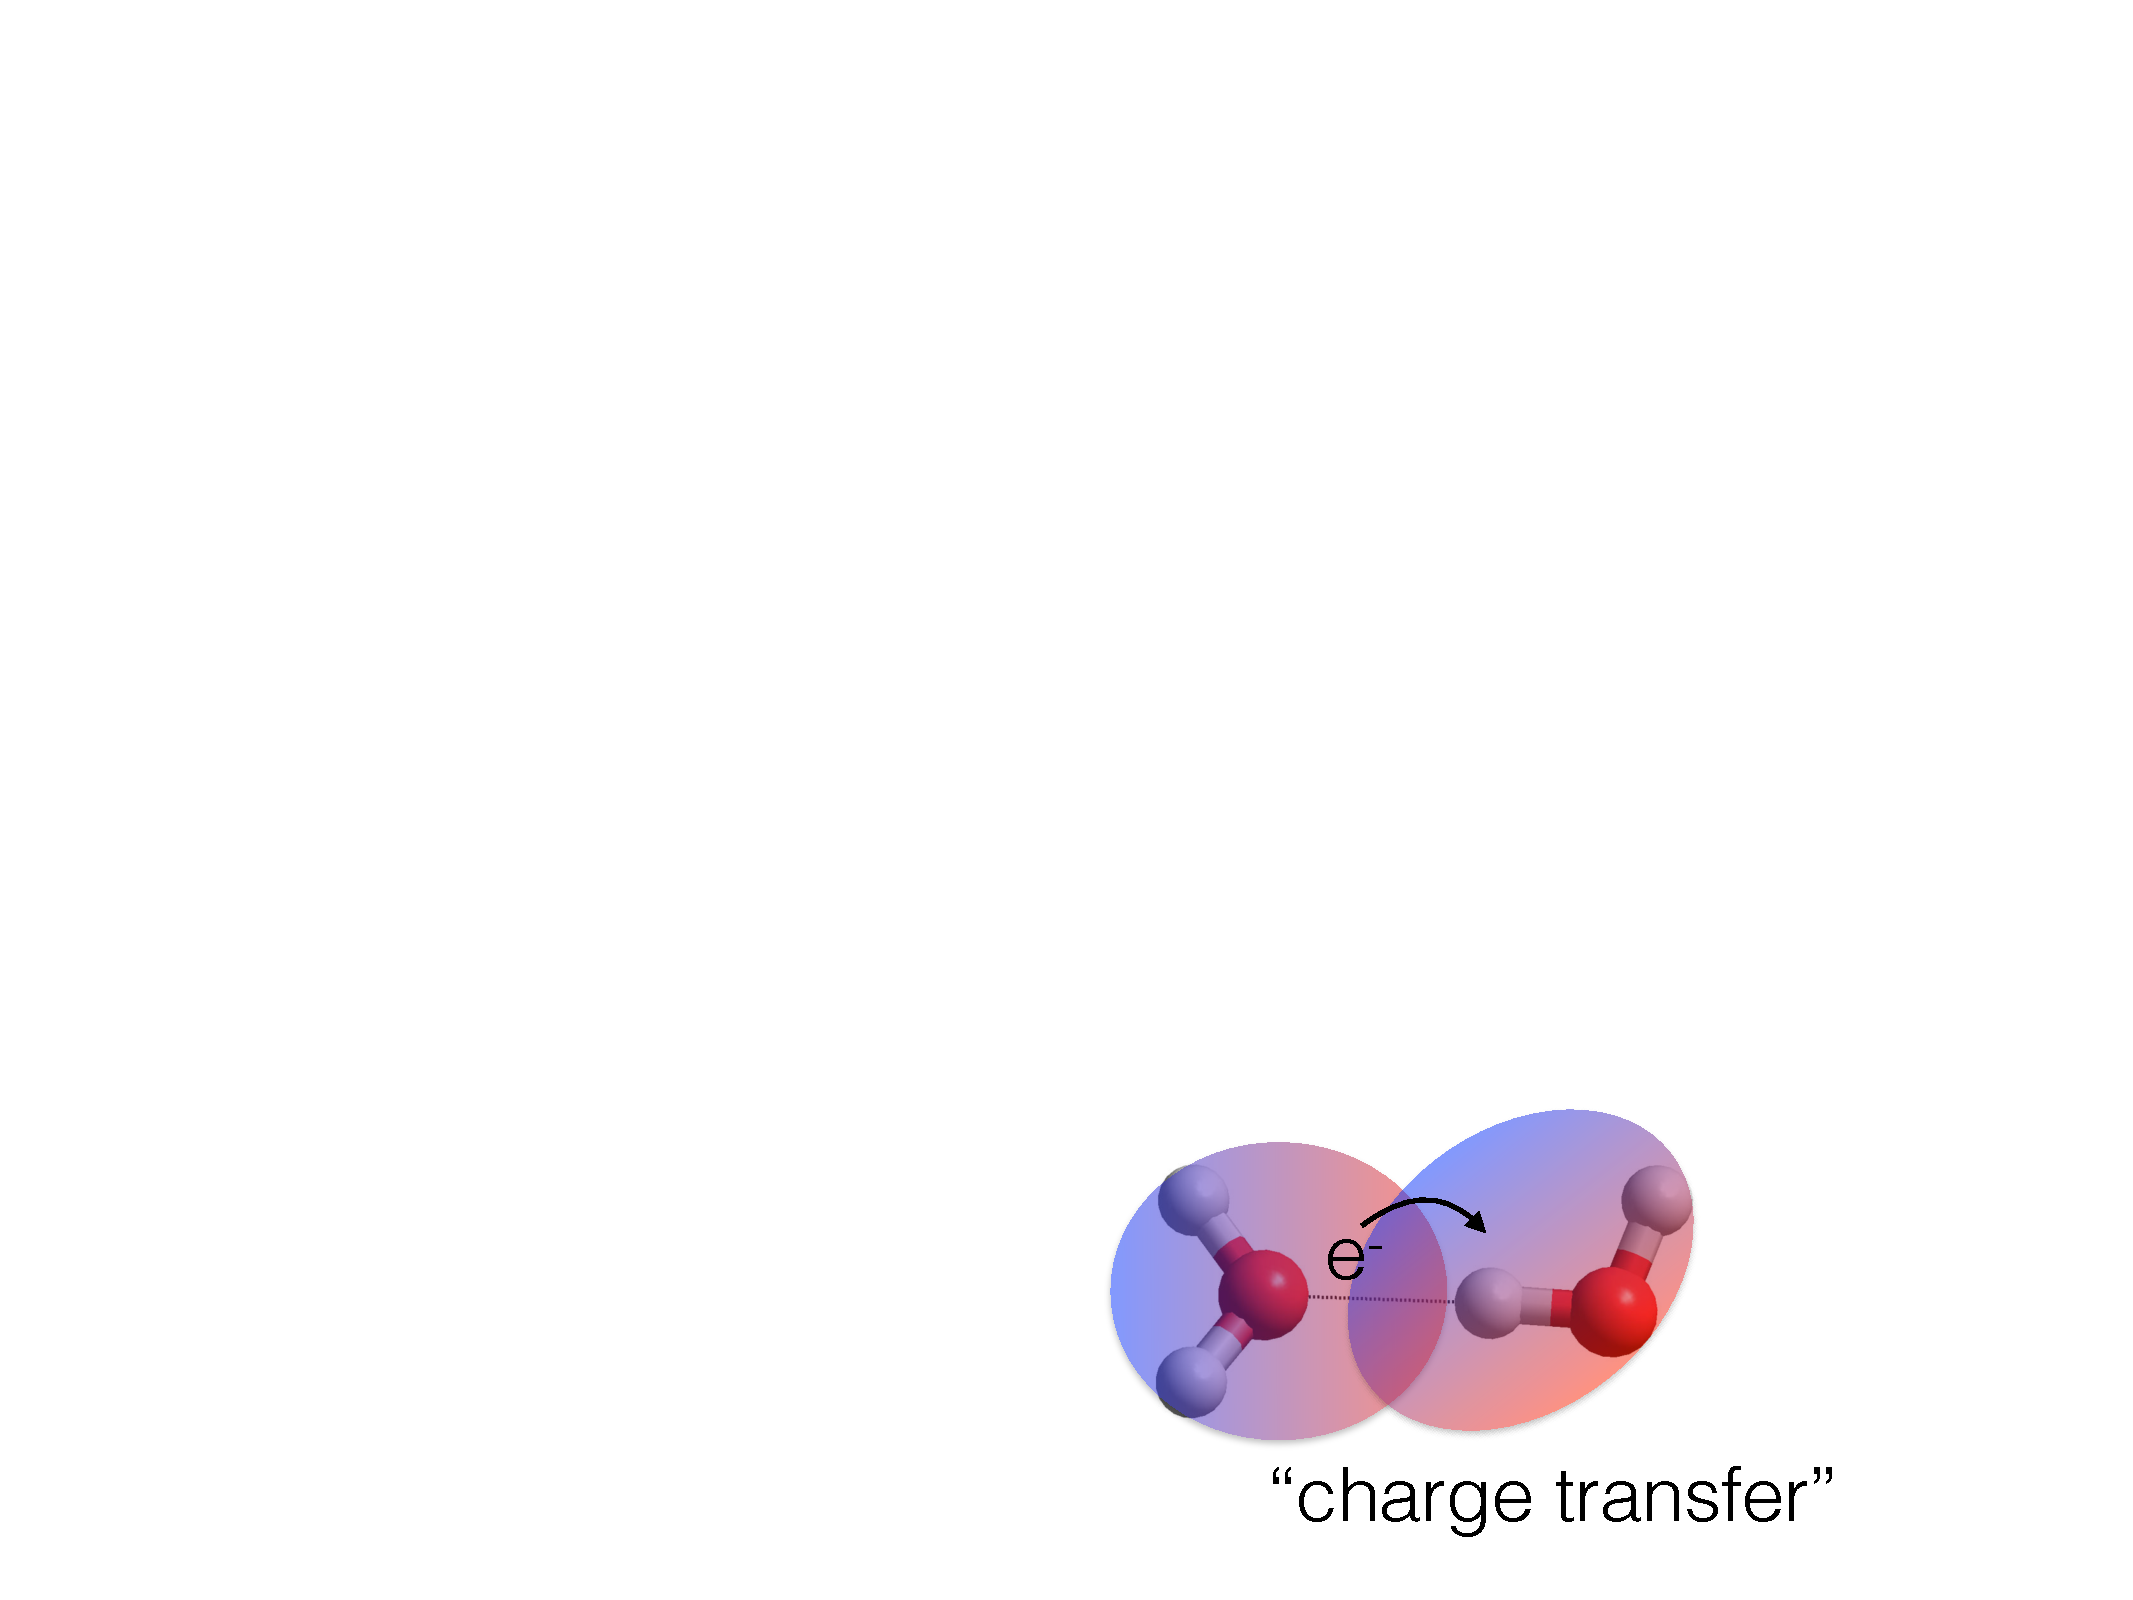
\includegraphics[scale=0.25]{./figures/almo_eda_04_ct.pdf}}
\end{frame}

\begin{frame}
  \frametitle{ALMO-EDA}
  \begin{equation*}
    \begin{aligned}
      \omega_{\text{tot}} &= \omega_{\text{free}} + \Delta \omega_{\text{int}} \\
      \Delta \omega_{\text{int}} &= \Delta \omega_{\text{gd}} + \Delta \omega_{\text{frz}} + \Delta \omega_{\text{pol}} + \Delta \omega_{\text{CT}}
    \end{aligned}
  \end{equation*}
\end{frame}

\begin{frame}
  \uncover<1->{\begin{equation*}
    E_{\text{tot}} = E_{\text{free}} + \Delta E_{\text{gd}} + \Delta E_{\text{frz}} + \Delta E_{\text{pol}} + \Delta E_{\text{CT}}
  \end{equation*}}
  \uncover<2->{\begin{equation*}
    \omega_{\text{tot}} = \omega_{\text{free}} + \Delta \omega_{\text{gd}} + \Delta \omega_{\text{frz}} + \Delta \omega_{\text{pol}} + \Delta \omega_{\text{CT}}
  \end{equation*}}
  \uncover<3->{\begin{equation*}
      \begin{aligned}
        \braket{\braket{\hat{P};\hat{Q}^{\omega}}}_{\text{tot}} = &\braket{\braket{\hat{P};\hat{Q}^{\omega}}}_{\text{free}} + \Delta \braket{\braket{\hat{P};\hat{Q}^{\omega}}}_{\text{gd}} \\
        &+ \Delta \braket{\braket{\hat{P};\hat{Q}^{\omega}}}_{\text{frz}} + \Delta \braket{\braket{\hat{P};\hat{Q}^{\omega}}}_{\text{pol}} + \Delta \braket{\braket{\hat{P};\hat{Q}^{\omega}}}_{\text{CT}}
    \end{aligned}
  \end{equation*}}
\end{frame}

\begin{frame}
  \centering
  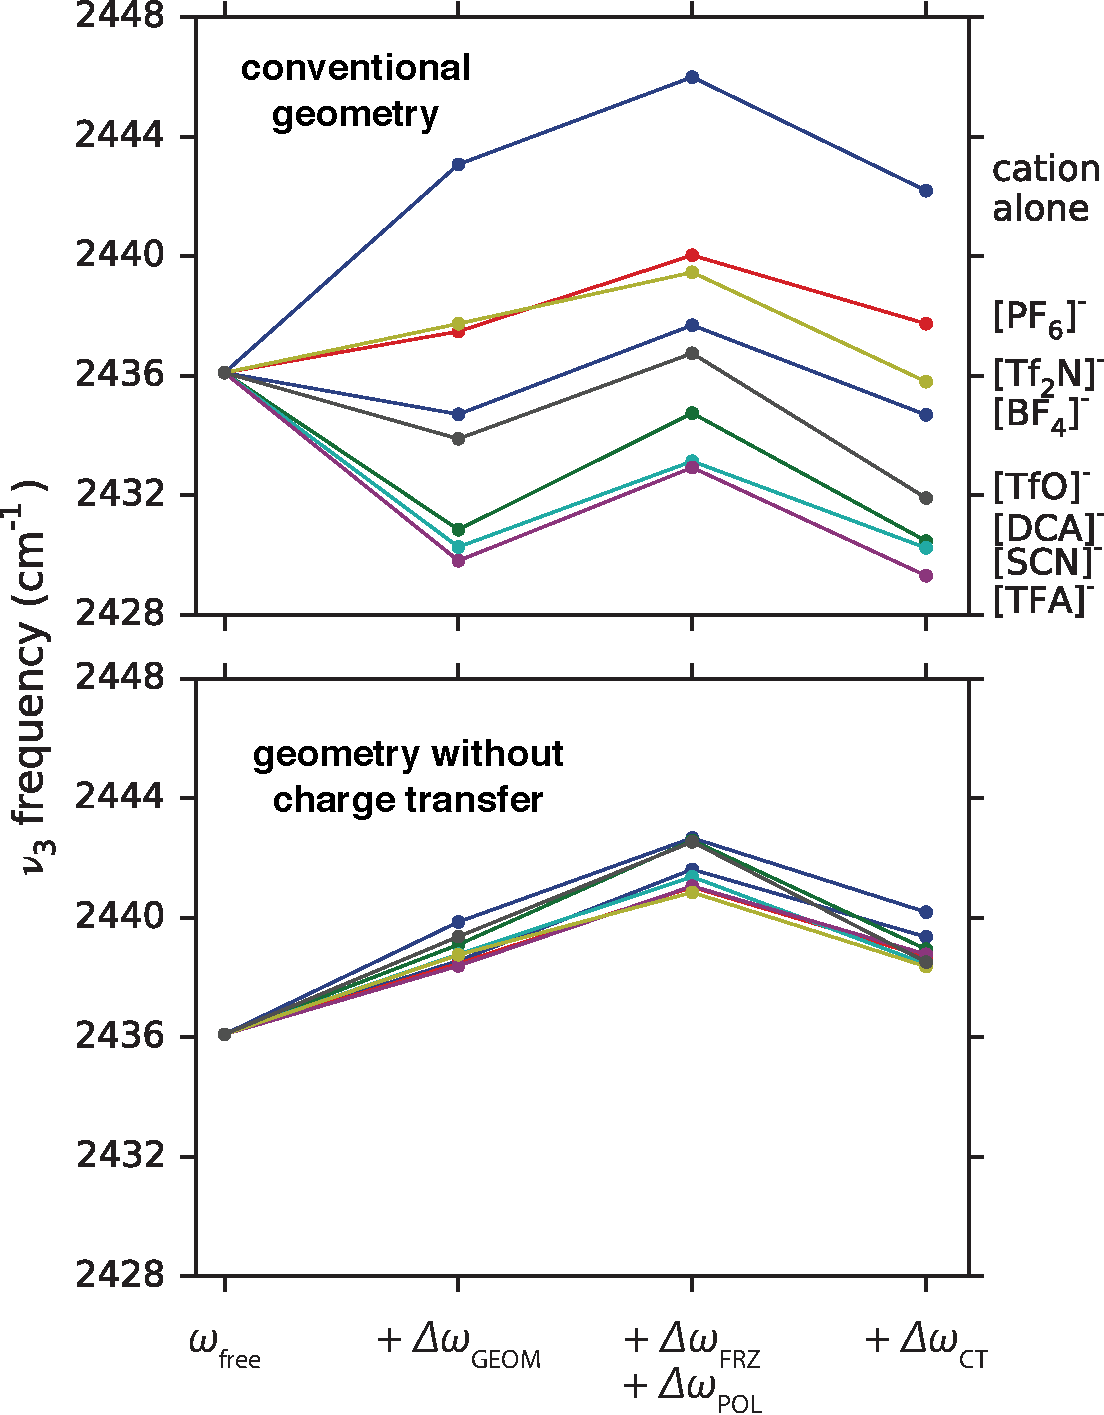
\includegraphics[scale=0.38]{./figures/ionic_liquid_geometry_dependence_on_ct.pdf}
\end{frame}

\begin{frame}
  \centering
  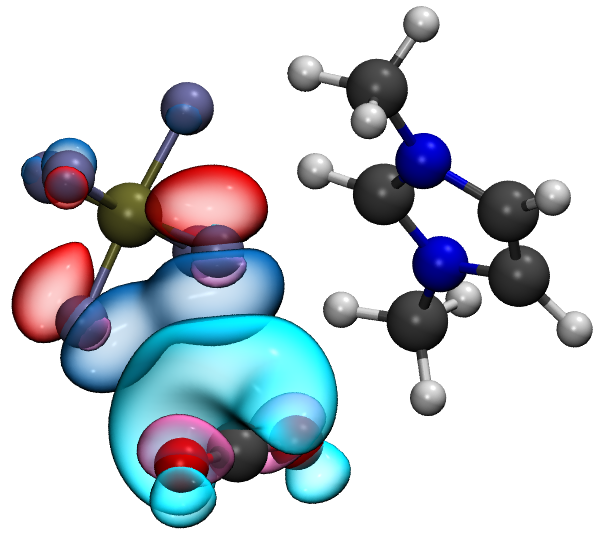
\includegraphics[scale=0.23,natwidth=601,natheight=535]{./figures/PF6.to_CO2.1.png}
  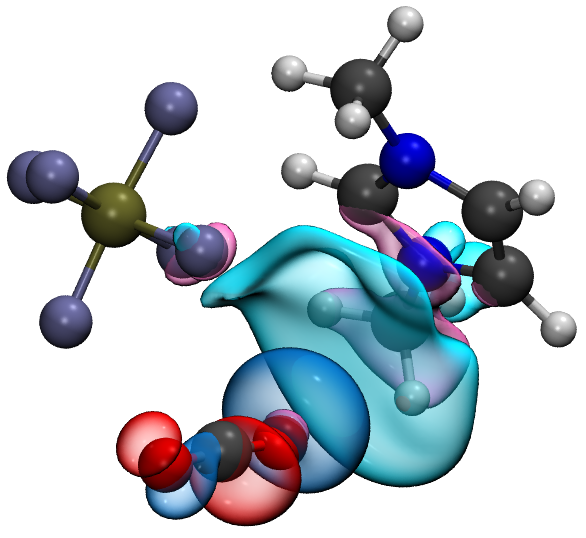
\includegraphics[scale=0.23,natwidth=586,natheight=538]{./figures/PF6.from_CO2.1.png}
\end{frame}

\begin{frame}
  \frametitle{Spectroscopic properties are directly connected to energy derivatives}
  \centering
  \scriptsize
  \begin{tabulary}{1.00\textwidth}{rL}
    \toprule
    \textbf{Derivative} & \textbf{Molecular property} \\
    \midrule
    \(\frac{dE}{dF_{i}}\)                          & dipole moment; similarly,  multipole moments, electric field gradients, etc. \\
    \(\frac{dE}{dB_{\alpha}}\)                     & magnetic dipole moment and higher-order magnetic multipoles \\
    \(\frac{dE}{dX_{i}}\)                          & forces on nuclei; stationary points on potential energy surfaces, equilibrium and transition state structures \\
    \(\frac{dE}{dm_{K_{j}}}\)                      & spin density; hyperfine interaction constants \\
    \textcolor{AlertColor}{\(\frac{d^{2}E}{dF_{\alpha}dF_{\beta}}\)}       & \textcolor{AlertColor}{polarizability} \\
    \textcolor{AlertColor}{\(\frac{d^{2}E}{dX_{i}dX_{j}}\)}                & \textcolor{AlertColor}{harmonic force constants and vibrational frequencies} \\
    \(\frac{d^{2}E}{dX_{i}dF_{\alpha}}\)           & dipole derivatives; harmonic infrared intensities \\
    \(\frac{d^{2}E}{dB_{\alpha}dB_{\beta}}\)       & magnetizability \\
    \(\frac{d^{2}E}{dm_{K_{j}}dB_{\alpha}}\)       & nuclear magnetic shielding tensor; relative NMR shifts \\
    \(\frac{d^{2}E}{dI_{K_{i}}dI_{L_{j}}}\)        & indirect spin-spin coupling constant \\
    \(\frac{d^{2}E}{dB_{\alpha}dJ_{\beta}}\)       & rotational \textit{g}-tensor; rotational spectra in magnetic field \\
    \(\frac{d^{2}E}{dI_{K_{i}}dB_{\alpha}}\)       & nuclear spin-rotation tensor; fine structure in rotational spectra \\
    \(\frac{d^{2}E}{dS_{i}dB_{\alpha}}\)           & electronic \textit{g}-tensor \\
    % \(\frac{d^{3}E}{dX_{i}dF_{\alpha}dF_{\beta}}\) & polarizability derivative; Raman intensities \\
    % \(\frac{d^{3}E}{dF_{\alpha}d^{2}F_{\beta}}\)   & (first) electric hyperpolarizability \\
    % \(\frac{d^{3}E}{dX_{i}dX_{j}dX_{k}}\)          & cubic force constants; vibrational corrections to distances and rotational constants \\
    % \(\frac{d^{4}E}{dF_{\alpha}dF_{\beta}dF_{\gamma}dF_{\delta}}\) & (second) electric hyperpolarizability \\
    % \(\frac{d^{4}E}{dB_{\alpha}dB_{\beta}dB_{\gamma}dB_{\delta}}\) & (second) hypermagnetizability \\
    % \(\frac{d^{4}E}{dX_{i}dX_{j}dX_{k}dX_{l}}\)                    & quartic force constants; anharmonic corrections to vibrational frequencies \\
    % \(\frac{d^{4}E}{dF_{\alpha}dF_{\beta}dF_{\gamma}dX_{i}}\)      & hyper-Raman effects \\
    % \(\frac{d^{4}E}{dF_{\alpha}dF_{\beta}dX_{i}dX_{j}}\)           & Raman intensities for overtone and combination bands \\
    % \(\frac{d^{4}E}{dF_{\alpha}dF_{\beta}dB_{\gamma}dB_{\delta}}\) & Cotton\textendash{}Mutton effect \\
    ... & ... \\
    \bottomrule
  \end{tabulary}
\end{frame}

\begin{frame}
  \frametitle{Quick-and-dirty linear response}
  The response of the property \(\hat{P}\) to the perturbation \(\hat{Q}\); for exact (orthogonal) states:
  \begin{equation*}
    \braket{\braket{\hat{P};\hat{Q}}}_{\omega_{Q}} = - \sum_{n>0} \left[ \frac{\braket{0|\hat{P}|n}\braket{n|\hat{Q}|0}}{\omega_{n} - \omega_{Q}} + \frac{\braket{0|\hat{Q}|n}\braket{n|\hat{P}|0}}{\omega_{n} + \omega_{Q}} \right]
  \end{equation*}
  where \(\omega_{n} = E_{n} - E_{0}\). For single-configuration methods in the static limit (\(\omega_{Q} = 0\)),
  \begin{equation*}
    \braket{\braket{\hat{P}_{\alpha};\hat{Q}_{\beta}}}_{0} = - \vect{P}_{\alpha}^{\dagger} \vect{G}^{-1} \vect{Q}_{\beta}
  \end{equation*}
  where
  \begin{equation*}
    (\vect{P}_{\alpha})_{ia} = -2 \braket{ i | \hat{P}_{\alpha} | a }
  \end{equation*}
  is a vector of property integrals in the occupied-virtual MO basis and \(\vect{G}^{-1}\) is the inverted orbital Hessian. The key step is forming the response vector
  \begin{equation*}
    X_{ia} = G_{ia,jb}^{-1} Q_{jb}.
  \end{equation*}
  \(X_{ia}\) is equivalent to the orbital rotation matrix \(U_{ia}\) from coupled perturbed SCF (CPHF, CPKS).
\end{frame}

\begin{frame}
  \frametitle{Spectroscopic properties are directly connected to response functions}
  \centering
  \begin{tabular}{ll}
    \toprule
    \textbf{Molecular property}       & \textbf{Linear response function} \\
    \midrule
    polarizability                    & \( \braket{\braket{\hat{\mu};\hat{\mu}}}_{\omega} \) \\
    magnetizability                   & \( \braket{\braket{\hat{m};\hat{m}}}_{0} \) \\
    optical rotation                  & \( \braket{\braket{\hat{\mu};\hat{m}}}_{\omega} \) \\
    electronic circular dichroism     & \( \braket{\braket{\hat{\mu};\hat{m}}}_{\omega_{f}} \) \\
    IR intensities                    & \( \braket{\braket{\hat{\mu};\partial\hat{H}_{0}/\partial R}}_{\omega} \) \\
    NMR spin-spin coupling constants  & \( \braket{\braket{\hat{h}_{\text{SD}};\hat{h}_{\text{SD}}}}_{0} \), \\
                                      & \( \braket{\braket{\hat{h}_{\text{FC}};\hat{h}_{\text{FC}}}}_{0} \), \\
                                      & \( \braket{\braket{\hat{h}_{\text{PSO}};\hat{h}_{\text{PSO}}}}_{0} \) \\
    NMR chemical shifts               & \( \braket{\braket{\hat{l}_{O};\hat{h}_{\text{PSO}}}}_{0} \) \\
    EPR \textit{g}-tensor             & \( \braket{\braket{\hat{l}_{O};\hat{h}_{\text{SOC}}}}_{0} \) \\
    ... & ... \\
    \bottomrule
  \end{tabular}
\end{frame}

% \begin{frame}[fragile]
%   \frametitle{An Algorithm For Finding Primes Numbers.}
% \begin{semiverbatim}
% \uncover<1->{\alert<0>{int main (void)}}
% \uncover<1->{\alert<0>{\{}}
% \uncover<1->{\alert<1>{  \alert<4>{std::}vector<bool> is_prime (100, true);}}
% \uncover<1->{\alert<1>{  for (int i = 2; i < 100; i++)}}
% \uncover<2->{\alert<2>{    if (is_prime[i])}}
% \uncover<2->{\alert<0>{      \{}}
% \uncover<3->{\alert<3>{        \alert<4>{std::}cout << i << " ";}}
% \uncover<3->{\alert<3>{        for (int j = i; j < 100;}}
% \uncover<3->{\alert<3>{             is_prime [j] = false, j+=i);}}
% \uncover<2->{\alert<0>{      \}}}
% \uncover<1->{\alert<0>{  return 0;}}
% \uncover<1->{\alert<0>{\}}}
% \end{semiverbatim}

%   \visible<4->{Note the use of \alert{\texttt{std::}}.}
% \end{frame}

% \begin{frame}
% \end{frame}


\begin{frame}
  \frametitle{Example: Static polarizability}
  As an energy derivative,
  \begin{equation*}
    \alpha_{rs} = - \left. \frac{\text{d}^{2}E}{\text{d}F_{r}\text{d}F_{s}} \right|_{\mathbf{F}=\mathbf{0}}
  \end{equation*}
  which is equivalent to the response theory formulation
  \begin{equation*}
    \alpha_{rs} = - \braket{\braket{\hat{\mu}_{r};\hat{\mu}_{s}}}_{0}.
  \end{equation*}
\end{frame}

\begin{frame}
  \frametitle{Acknowledgements}
  \begin{columns}
    % \column{0.35\textwidth}
    % \begin{itemize}
    % \item Evgeny Epifanovsky
    % \item Q-Chem
    % \item Adrian Morrison
    % \item Daniel Lambrecht
    % \end{itemize}
    % \column{0.65\textwidth}
    % \begin{center}
    %   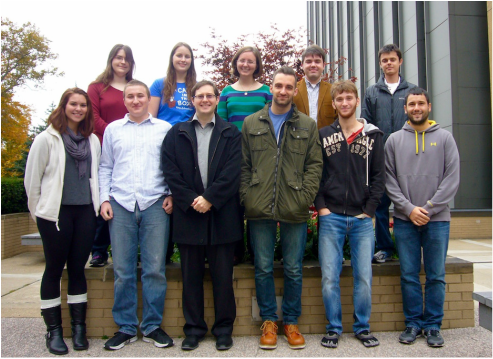
\includegraphics[scale=0.40]{./images/lambrecht_group.png} \\
    %   
\includegraphics[scale=0.40]{./images/pitt_logo.pdf}
    % \end{center}
    \column{0.65\textwidth}
    \begin{minipage}{1.0\linewidth}
      \begin{itemize}
      \item Prof. Daniel Lambrecht
      \item Prof. Sean Garrett-Roe
      \item Prof. Ken Jordan
      \item Evgeny Epifanovsky (Q-Chem)
      \item Daniel Smith (MolSSI, Psi4)
      \item Tom Brinzer
      \end{itemize}
    \end{minipage}
    \column{0.35\textwidth}
    \begin{minipage}{1.0\linewidth}
      \centering
      
\includegraphics[width=1.00\linewidth,keepaspectratio]{./figures/Qchem-logo.png}
      
\includegraphics[width=0.90\linewidth,keepaspectratio]{./figures/PQI-Letter-Logo-black.png}
      
\includegraphics[width=0.85\linewidth,keepaspectratio]{./figures/logo_crc.jpg}
      
\includegraphics[width=0.95\linewidth,keepaspectratio]{./figures/logo_novartis.png}
      
\includegraphics[scale=0.15]{./figures/logo_cclib.png}
      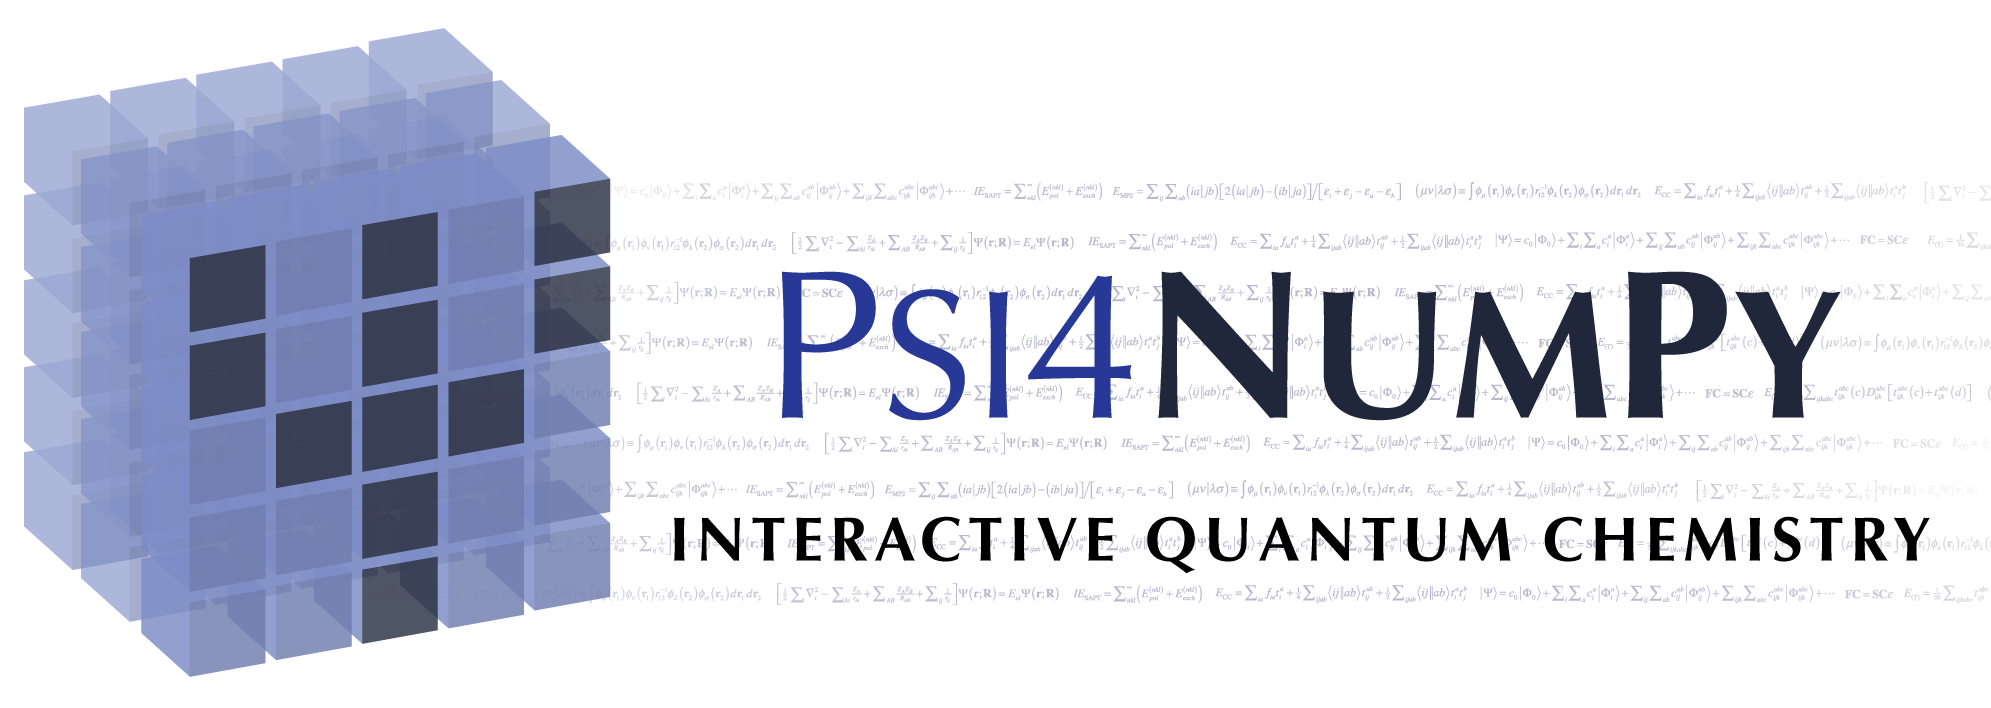
\includegraphics[width=1.00\linewidth,keepaspectratio]{./figures/psi4numpybanner_eqn.png}
      
\includegraphics[width=0.95\linewidth,keepaspectratio]{./figures/logo_molssi_text.jpg}
    \end{minipage}
  \end{columns}
\end{frame}

\begin{frame}
  \frametitle{Thank you}
  \scriptsize
  \begin{enumerate}
  \item \fullcite{Berquist2014}
  \item \fullcite{Shao2015}
  \item \fullcite{Brinzer2015}
  \item \fullcite{Daly2016}
  \item \fullcite{Berquist2017}
  \item \fullcite{Brinzer2017}
  \item \fullcite{Smith2018}
  \item \fullcite{Berquist2018}
  \item \fullcite{Jakubek2018}
  \end{enumerate}
\end{frame}

\begin{frame}
  \frametitle{Extra slides}
\end{frame}

\begin{frame}
  \frametitle{Implementation: working equations (RHF)}
  \begin{align*}
    \Delta_{ia} &= \epsilon_{a} - \epsilon_{i} \\
    A_{ia,jb}^{s} &= \Delta_{ia}\delta_{ia,jb} + 2(ia|jb) - (ij|ab) \\
    B_{ia,jb}^{s} &= 2(ia|jb) - (ib|ja) \\
    A_{ia,jb}^{t} &= \Delta_{ia}\delta_{ia,jb} - (ij|ab) \\
    B_{ia,jb}^{t} &= - (ib|ja) \\
    ^{\text{RR}}\vect{G}^{uu} &= (\vect{A}^{u} + \vect{B}^{u}) \\
    ^{\text{II}}\vect{G}^{uu} &= (\vect{A}^{u} - \vect{B}^{u})
  \end{align*}
  \scriptsize
  \begin{itemize}
  \item \(\vect{G}\) gives orbital rotation Hessians, equivalen to the random phase approximation (RPA) equations \\
  \item R, I: real, imaginary perturbations \(\rightarrow\) electric and magnetic Hessians \\
  \item setting \(\vect{B} = \vect{0}\) gives the Tamm-Dancoff approximation (TDA) \\
  \item setting \( G_{ia,jb} = (\epsilon_{a} - \epsilon_{i})\delta_{ia,jb} \) gives uncoupled Hartree-Fock \\
  \item \(s,t\): singlet (spin-conserving) and triplet (altering) operators \\
  \item \(i,j\): occupied MOs, \(a,b\): virtual MOs
  \end{itemize}
\end{frame}

\begin{frame}
  \frametitle{Implementation: AO-direct algorithm}
  Rather than explicitly forming \(G_{ia,jb}\), inverting it, and contracting with \(Q_{jb}\) to form the response vector \(X_{ia}\), the solution is found iteratively (example is RPA/singlet):
  \begin{equation*}
    X_{ia}^{(\zeta+1)} \leftarrow \frac{Q_{jb} - \left[4(ia|jb) - (ij|ab) - (ib|ja)\right] X_{jb}^{(\zeta)}}{\Delta_{ia}}
  \end{equation*}
  The uncoupled result comes from the initial guess, when \(X_{ia}^{(0)} = 0\):
  \begin{equation*}
    X_{ia}^{(1)} = \frac{Q_{ia}}{\Delta_{ia}}
  \end{equation*}
  Convergence is usually accelerated with CG, DIIS, ...
\end{frame}

\begin{frame}
  \frametitle{Implementation: AO-direct algorithm}
  \scriptsize
  The key step in each iteration is forming the matrix-vector product
  \begin{equation*}
    (\vect{A}+\vect{B})_{ia,jb}X_{jb} = \left[4(ia|jb) - (ij|ab) - (ib|ja)\right] X_{jb}^{(\zeta)}
  \end{equation*}
  which is found through back-transforming to the AO basis, starting from the generalized density:
  \begin{equation*}
    D_{\lambda\sigma}^{X} \equiv C_{\lambda j} X_{jb} C_{\sigma b}
  \end{equation*}
  which is contracted with two-electron integrals formed either exactly or through approximate methods (RI, ...):
  \begin{align*}
    (\vect{A}+\vect{B})_{ia,jb}X_{jb} &= C_{\mu i} \left\{ 4(\mu\nu|\lambda\sigma)D_{\lambda\sigma}^{X} - (\mu\lambda|\nu\sigma)D_{\lambda\sigma}^{X} - (\mu\sigma|\lambda\nu)D_{\lambda\sigma}^{X} \right\} C_{\nu a} \\
    &= C_{\mu i} \left\{ 4J_{\mu\nu}^{X} - K_{\mu\nu}^{X} - K_{\nu\mu}^{X} \right\} C_{\nu a}
  \end{align*}
  In \texttt{libint}, this is \texttt{JobNum = 30}.
\end{frame}

\begin{frame}[fragile]
  \frametitle{Implementation: library usage}
  \texttt{responseman} is a thin wrapper around \texttt{libresponse}, and is not meant to calculate final properties (similar to \texttt{**RESPONSE} vs. \texttt{**PROPERTIES} in DALTON). \\
  \begin{minted}[linenos,gobble=0,mathescape]{c++}
    void solve_linear_response(
        arma::cube &results,
        MatVec_i *matvec,
        arma::cube &C,
        arma::mat &moene,
        arma::uvec &occupations,
        std::vector<double> &omega,
        arma::cube &V,
        std::vector<int> &b_prefactors,
        libresponse::configurable &cfg
    );
  \end{minted}
\end{frame}

\begin{frame}[fragile]
  \frametitle{Implementation: integral engine}
  \scriptsize
  \begin{minted}[linenos,gobble=0,mathescape]{c++}
if (ints_engine == "libfock" || ints_engine == "both") {
    matvec_libfock = new MatVec_libfock();
    libqints::basis_1e1c_cgto<double> b1;
    libqints::qchem::bagen_1e1c_cgto_qchem(b1);
    matvec_libfock->init(b1, mem_mb);
    matvec = matvec_libfock;
} else if (ints_engine == "qchem" || ints_engine == "both") {
    matvec_qchem = new MatVec_qchem();
    matvec_qchem->init();
    matvec = matvec_qchem;
} else
    ...
  \end{minted}
\end{frame}

\begin{frame}
  \frametitle{Hardware and software}
  \begin{itemize}
  \item CPU: Intel Xeon E5-2670 (Sandy Bridge), 2.60 GHz, 16 cores
  \item DALTON 2015.0; Intel 2013.0
  \item ORCA 3.0.3
  \item Q-Chem \texttt{branches/libresponse r21370} with \texttt{libresponse r72}, \texttt{libqints r1058}, \texttt{libfock r198}; Intel 2015.1
  \item \texttt{scf\_convergence = 9}, \texttt{thresh = 12}, \texttt{cpscf\_max\_error\_norm = 14}
  \end{itemize}
\end{frame}

\begin{frame}
  \frametitle{Current capabilities}
  QC methods:
  \begin{itemize}
  \item RHF, UHF references \(\rightarrow\) DALTON is ROHF, is this the first true general UHF linear response code?
  \item Hartree-Fock via \texttt{libfock/libqints} or \texttt{libint}
  \end{itemize}
  Operators (\texttt{libint}):
  \begin{itemize}
  \item dipole (length), quadrupole at arbitrary origin
  \item Fermi contact at nuclear positions
  \item dipole velocity/linear momentum
  \item angular momentum at arbitrary origin
  \item one-electron spin-orbit over all nuclei w/ arbitrary charges
  \end{itemize}
  Properties via \texttt{responseman}:
  \begin{itemize}
  \item static polarizability
  \end{itemize}
\end{frame}

\begin{frame}
  \frametitle{Planned capabilities}
  \begin{itemize}
  \item Convergence acceleration (DIIS via \texttt{libsolve})
  \item DFT via \texttt{libint/dftman} \(\rightarrow\) all functionals should work
  \item Operators: two-electron spin-orbit, arbitrary-order electric field multipoles at arbitrary origin, spin dipole at nuclear positions
  \item time-dependent/dynamic properties
  \item residues \(\rightarrow\) transition moments
    \begin{equation*}
      \lim_{\omega_{1} \to \omega_{n0}} (\omega_{n0} - \omega_{1}) \braket{\braket{\hat{P};\hat{Q}^{\omega_{1}}}} = \braket{0|\hat{P}|n} \braket{n|\hat{Q}^{\omega_{1}}|0}
    \end{equation*}
  \item complex response via \texttt{gen\_scfman}
    \begin{equation*}
    \braket{\braket{\hat{P};\hat{Q}}}_{\omega_{Q}} = \sum_{n>0} \left[ \frac{\braket{0|\hat{P}|n}\braket{n|\hat{Q}|0}}{\omega_{n} - \omega_{Q} - i\gamma_{n0}} + \frac{\braket{0|\hat{Q}|n}\braket{n|\hat{P}|0}}{\omega_{n} + \omega_{Q} + i\gamma_{n0}} \right]
    \end{equation*}
  \item quadratic response \(\braket{\braket{\hat{P};\hat{Q},\hat{R}}}_{\omega_{Q},\omega_{R}}\)
  \item ALMO...
  \end{itemize}
\end{frame}

\end{document}
